%-----------------------------------------------------------------------------
%
%               Template for sigplanconf LaTeX Class
%
% Name:         sigplanconf-template.tex
%
% Purpose:      A template for sigplanconf.cls, which is a LaTeX 2e class
%               file for SIGPLAN conference proceedings.
%
% Guide:        Refer to "Author's Guide to the ACM SIGPLAN Class,"
%               sigplanconf-guide.pdf
%
% Author:       Paul C. Anagnostopoulos
%               Windfall Software
%               978 371-2316
%               paul@windfall.com
%
% Created:      15 February 2005
%
%-----------------------------------------------------------------------------


\documentclass[smallextended]{svjour3} 

% The following \documentclass options may be useful:

% preprint      Remove this option only once the paper is in final form.
% 10pt          To set in 10-point type instead of 9-point.
% 11pt          To set in 11-point type instead of 9-point.
% authoryear    To obtain author/year citation style instead of numeric.

\usepackage{amsmath}
\usepackage{tikz}
\usepackage{pgfplots}
\pgfplotsset{compat=1.3}
\usepackage{graphicx, epsfig}
\usepackage{xspace}  %% Package used for the \NB{} abbreviation
\usepackage{algorithm}
\usepackage{algpseudocode}
\usepackage{color}
\usepackage{url}
\usepackage{hyperref}
\usepackage{listings}
\usepackage{tikz}% http://ctan.org/pkg/pgf
\usetikzlibrary{calc}
\usepackage{amssymb,amsmath}
\usepackage{subfigure}


\lstset{language=C++,
	basicstyle=\ttfamily\scriptsize, %aboveskip={-5ex},
	columns=fullflexible,
	%basicstyle={\ttfamily\singlespacing},aboveskip={-4ex},
	keywordstyle=\color{blue}\ttfamily,
	stringstyle=\color{red}\ttfamily,
	commentstyle=\color{cyan}\ttfamily,
	captionpos=t,
	%numbers=none, %left,
	numbers=left,
	%numberstyle=\scriptsize,
	%stepnumber=1,
	%numbersep=6pt,
	showstringspaces=false,
	breaklines=true,
	frame=lines,
	otherkeywords={[[,]],::,constexpr},
	emph={rpr,kernel,target,in,out,pipeline,stream,farm,pipe,map,sync,async, rprmv, base, split, unroll, Pipeline, Farm, parallel_execution_ff},
	emphstyle={\color{magenta}\bfseries}
}

\begin{document}


	\title{Programming Heterogeneous Parallel Machines using Refactoring and Monte-Carlo Tree Search}


\author{Christopher Brown         \and
	Vladimir Janjic  \and 
	M. Goli \and
	J. McCall \and
}

%\authorrunning{Short form of author list} % if too long for running head

\institute{C. Brown, V. Janjic \at
	School of Computer Science, University of St Andrews, UK. \\
	\email{\{cmb21,vj32\}@st-andrews.ac.uk}           %  \\
	%             \emph{Present address:} of F. Author  %  if needed
	\and
	M. Goli, J. McCall \at
	Robert Gordon University, Aberdeen, UK. \\
	\email{\{m.goli1, j.mccall\}@rgu.ac.uk}
}

\date{Received: date / Accepted: date}

%\author{\IEEEauthorblockN{Christopher Brown\IEEEauthorrefmark{1}, Vladimir Janjic\IEEEauthorrefmark{1}, Kevin Hammond\IEEEauthorrefmark{1}}
%\IEEEauthorblockA{\IEEEauthorrefmark{1}School of Computer Science\\
% University of St Andrews\\
% St Andrews\\
% United Kingdom\\E-Mail : \{cmb21,jv32,kh8\}@st-andrews.ac.uk}
%University of St Andrews, St Andrews, UK\\E-Mail : \{cmb21,jv32,kh8\}@st-andrews.ac.uk}
%\and
%\IEEEauthorblockN{Mehdi Goli\IEEEauthorrefmark{2}, John McCall\IEEEauthorrefmark{2}}
%\IEEEauthorblockA{\IEEEauthorrefmark{2}School of Computer Science\\
%Robert Gordon University,
%Aberdeen, UK
%\\E-Mail : \{m.goli1,j.mccall\}@rgu.ac.uk}}

% make the title area
\maketitle

\begin{abstract}
This paper presents a new technique for 
introducing and tuning parallelism for heterogeneous shared-memory systems (comprising a
mixture of CPUs and GPUs), using a combination of algorithmic skeletons (such as farms and pipelines),
Monte-Carlo tree search for deriving mappings of tasks to available hardware resources, and refactoring
tool support for applying the patterns and mappings in an easy and effective way.
Using our approach, we demonstrate easily obtainable, significant and scalable speedups on a number of case studies showing speedups of up to 41 over the sequential code on a 24-core machine
with one GPU. We also demonstrate that 
the speedups obtained by mappings derived by the MCTS algorithm are comparable to
the best possible speedups that can be obtained. %  for the particular application.
\keywords{Heterogeneous Parallel Computing; Monte-Carlo Tree Search; Optimisations}
\end{abstract}

\section{Introduction}

\textbf{Points to address in the final version}
\begin{itemize}
    \item For instance, instead of tuning the two parameters at a time, we could tune the parameters one by one using an assumption that the other parameter can be easily estimated with cheaper cost model. With this technique, the search space reduces from $n^2$ to $2n$ (let n be the number of possible values for each parameter).  The authors should compare MCTS with these simple but acceptable techniques, with experiments, at least.
    
    \emph{We can pull the results for hill-climbing, random sampling and exhaustive search from the other paper. Maybe re-run the programs to get all the mappings and also implement the method the reviewer proposed here}
    
    \item Another issue about MCTS is that there should be some adaptation of the algorithm to the proposed framework. Since MCTS is a game-search technique, the output is a single move at the root position.  However, the authors explain that whole set of parameters are obtained with MCTS.
    
    \emph{This should be quite straightforward. We just need to explain what the output of one run of the MCTS is a bit better.}
    
    \item Also, it
is unclear which measure is used in the selection step (usually UCB1 is used to maximize the expected win ratio) and which measure is used in the propagation step (usually MCTS keeps track the win/playout counts to evaluate win ratio and UCB1 value).  These algorithmic details should be properly addressed.

    \emph{Look at the CEC paper and pull out some data from there. I think this is mantioned there.}
    
    \item The last issue is about the evaluation of the MCTS part.  The quality of outputs depends on the number of playouts. The experiments given in the paper does not clarify this point.  Even the numbers of playouts for obtaining the experiment results are missing.
    
    \emph{We need to find the MCTS code for this.}
    
\end{itemize}

%% VJ: Check this over again
%%\subsection{To-Do List}
%\begin{itemize}
 %   \item The actual use of the refactoring tool is never shown; ToDo: Show a tool screenshot and code before and after the transofrmation? Or just explain the focus is not on refactoring tool...
  %  \item The authors claim that
%the approach is entirely generic and can be applied for different programming languages. ToDo: Clarify this. The general methodology could in principle be applied to different languages, but certain pieces of it (notably refactoring) depend on the syntax of the particular language, so they are C++ specific.
%    \item The experiments are based on C++ and the initial examples also show C++ code but the examples
%entirely omit the mechanics of the involved refactoring tool. There are only trivial examples
%of how the code looks like after the skeletons already got introduced. It is not clear to the reader
%to which degree this can be achieved automatically. ToDo: Explain that this can be done automatically.
 %   \item It would be desirable to provide additional
%information about the restrictions of the refactoring tool, as well as the degree to which users
%need to manually intervene. Are there differences between programming languages or does the
%tool work equally well for different languages? ToDo: Same as the above two points. Just play down the "completely generic" aspect a bit. 
%    \item The advantage of applying Monte-Carlo Tree Search algorithm is not discussed.
 %  At least we should discuss the advantages compared with genetic/evolutionary algorithms. ToDo: We can pick this up from the CEC paper.
  % \item
  % \item  The number of parameters is just 2 and the size of parameter space is quite small
  % to use Monte-Carlo Tree Search. In fact, if the number of parameters is 2 it should be unnecessary to use tree search algorithms. ToDo: Put some concrete numbers on the size of search space with different number of parameters. Also, explains that we are using profiling based methods to estimate the runtime of an app, so even if the search space is small, we still need to prune it.
  %% \item The detailed parameters in the Monte-Carlo Tree Search algorithms is missing, and thus
  % we cannot reproduce the results for further studies. ToDO: Also pull this from the CEC paper.
%\end{itemize}
%CB: scheduling vs. mapping
\noindent
Heterogeneous multicore systems are increasingly common.
% , comprising a mixture of CPUs and GPUs,
% , combining 
% dozens of CPU cores with hundreds of GPU cores.
Programming such systems remains difficult, however, since
common programming techniques, such as OpenCL or CUDA+OpenMP,
are very low level and 
require the programmer to make non-trivial scheduling and data-transfer decisions.
Moreover, applications generally have many sources of parallelism: deciding
which of the possible parallel structures should be exploited is especially challenging on heterogenous architectures.
%
In this paper, we introduce a new technique for programming heterogeneous parallel systems
that: \emph{i)} automatically discovers which parallel structure to exploit; \emph{ii)} computes a near-optimal mapping of work onto
the various heterogeneous processing elements; and, \emph{iii)} provides a semi-automatic way of
introducing the chosen parallel structure into the original program, and instantiating this with the derived mapping information.
Our technique is based on a combination of algorithmic skeletons~\cite{cole-th} for defining the parallel structure, % skeletons, 
 a method of finding a mapping for tasks on
 heterogeneous architectures%\footnote{Here we use Monte Carlo Tree Search (MCTS)~\cite{mc}.},
 and refactoring tool support for user-guided introduction of the skeletons and mapping decisions. 

We show the generality of our technique by using realistic 
use-cases from three different domains (image processing, 
heuristic optimisation and molecular dynamics), % showing the generality of our methodology.
% Our experiments on a 24-core shared-memory heterogeneous machine
% demonstrate that we are able to automatically derive parallel versions of applications that deliver speedups that can be within
% 5\% of the optimal speedup (over all possible parallel versions of the same application). 
programmed using the FastFlow~\cite{AldinucciDKMT11} skeleton library for C++, which uses OpenCL and CUDA for GPU computations. While some particular parts of the technology (e.g.~refactoring) necessarily depend on the syntax of C++ language, the general methodology could, in principle, be applied to other languages and paradigms (e.g.~Erlang~\cite{lapedo}).
%
The paper makes the following research contributions:
% \vspace{-12pt}
\begin{enumerate}
\item we introduce a new technique for building
  heterogeneous parallel programs semi-automatically, based on refactoring and algorithmic skeletons;
\item we introduce a mechanism for discovering
  efficient mappings of parallel application threads to heterogeneous CPU
  and GPU hardware, based on Monte-Carlo Tree Search simulations; and,
% VJ : This is not such a major contribution, if you ask me
%\item We define a precise specification for the static mapping problem; and,
% VJ : Since these refactorings are still manual, I would say that the
% static mapping stuff is a bigger contribution
%\item 
%We introduce a number of novel refactorings for introducing parallelism for heterogenous many-core systems, implemented in the CDT refactoring plugin for Eclipse;
\item we
%  evaluate our methodology on a number of realistic case studies from a number of domains, including image processing, 
% heuristic optimisation and molecular dynamics,
  show that, using our technique, 
  it is possible to derive a parallel structure and the corresponding mapping information, achieving
  performance that can be within 5\% of the best-obtained manual parallelisation.
\end{enumerate}

\section{Background} \label{sec:background}
%\subsection{Skeletons} \label{sec:skeletons}
\paragraph{Skeletons.} In this paper, we take a pattern-based approach, in which the parallel application is developed
by composing and/or nesting \emph{algorithmic skeletons}. An \emph{algorithmic skeleton}~\cite{cole-th} is an abstract
computational entity that models some common pattern of computation. % parallelism (as described below).
A skeleton is typically implemented as a higher-order function that abstracts over low-level details such as 
thread creation, communication, synchronisation, load balancing, etc.
%In this paper, w
We consider two categories of skeletons: \emph{sequential} skeletons, abstracting
the structure of a purely sequential computation with no added parallelism; and, \emph{parallel}
skeletons, which implement specific parallel patterns. In our skeleton definitions, we assume
that all of the input tasks are independent.
We consider two \emph{sequential} skeletons:
\begin{itemize}
\item The \emph{Compose ($\circ$)} skeleton represents sequential
  function composition applied to a sequence of inputs, where
$f1 \circ f2$ denotes a sequential composition of two functions, $f1$ and $f2$.
\item The \emph{Order ($;$)} skeleton represents the execution of two
 functions on a sequence of inputs, where the execution of the first function needs to be
 completed for all input values before the execution of the second one
 can start. $f ; g$, therefore, requires synchronisation
 between $f$ and $g$.
\end{itemize}

We also consider two widely-used parallel skeletons:
\begin{itemize}
\item The \emph{Pipeline ($\parallel$)} skeleton applies
    the composition
    of the functions \\ $f_1, f_2, \dots, f_n$, \emph{in parallel} to a sequence of independent inputs
   $x_1,x_2,\dots,x_m$, where the output of $f_i$ is the input to
   $f_{i+1}$. Parallelism arises from the fact that
   $f_i(x_j)$ can be computed in parallel with
   $f_{i+1}(f_i(x_{j-1}))$. In the implementation that we
   consider, a separate thread is assigned to each
   \emph{pipeline stage} (function $f_i$).
   We denote the pipeline skeleton by
    $(f_1 \parallel f_2 \parallel \dots \parallel f_n)(x) $.
\item A \emph{Farm ($\Delta$)} skeleton,  $\Delta(\mathit{nwCPU},\mathit{nwGPU},f,x)$, represents the application of a single function,
  $f$, to the sequence of independent inputs,\\ 
  $x_1,x_2,x_3,\dots,x_n$, in parallel. In the farm implementation
  that we consider, a specific number of
  \emph{worker threads} is created, and the inputs are assigned to
  these worker threads in a round-robin fashion.  
 Here \emph{nwCPU}/\emph{nwGPU} are, respectively, the number of worker
  threads executed on CPUs/GPUs.
\end{itemize}

\noindent
We also allow nested skeletons. It is, therefore, possible to, for example, nest a
pipeline inside a farm,\ $\Delta(nwCPU,nwGPU,f1 \parallel f2, x)$.
A \emph{skeletal configuration}  abstracts over the skeleton
parameters (e.g. the number and type of
workers in a farm), thus focusing only on the nesting structure of the
skeletons. In a skeletal configuration, we denote
$\Delta(\mathit{nwCPU},\mathit{nwGPU},f,x)$ simply by $\Delta(f)$, and $(f_1 \parallel
f_2 \parallel \dots \parallel f_n)(x)$ by $f_1 \parallel f_2
\dots \parallel f_n$. For example, the skeletal
configuration $\Delta(f) \parallel (g \circ \Delta(h))$
denotes a
pipeline of two stages, % where the first stage is
i) a farm whose worker function is $f$, and ii) a sequential composition of
function $g$ with a farm whose worker function is $h$. % denoted by
%
% In this paper we use the FastFlow~\cite{AldinucciDKMT11}  skeleton library for C++
% for the implementation of these skeletons.

%\subsection{Refactoring}
\paragraph{Refactoring}
Refactoring is the process of changing the structure of a program
while preserving its functional semantics in order, for example, 
to increase code quality, programming productivity and code reuse.
The term \emph{refactoring} was first introduced by Opdyke in his PhD
thesis in 1992~\cite{opdyke}, and the concept goes back at least to the fold/unfold system proposed
by Burstall and Darlington in 1977~\cite{darlington77}.
Refactoring is a \emph{semi-automatic} approach that is much more
general than fully automated parallelisation techniques, which typically
only work for a very limited range of cases under limited conditions.
Additionally, unlike simple loop parallelisation, refactoring is applicable
to a much wider range of possible parallel structures, since the parallelism is introduced
in a controlled way via skeletons.
In this paper we make use of a refactoring extension~\cite{pdp} for Eclipse, that introduces and tunes parallelism in C++ by introducing a nesting of skeletons into the application semi-automatically by user-guidance.
%\subsection{FastFlow}
%\noindent
%FastFlow~\cite{AldinucciDKMT11} is a skeleton-based parallel programming framework
%for multi-core platforms, implemented in C++.
%% . FastFlow facilitates the development
%% of shared-memory parallel applications by providing
%% abstraction layers, programming constructs, and composable
%% algorithmic skeletons~\cite{AldinucciDKMT11}.
%FastFlow's streaming patterns are coordinating mechanisms
%that control the flow of work between multiple concurrent
%threads. This allows programmers to focus on
%application-specific computational components by
%abstracting over complex coordination and communication
%layers. 
%FastFlow supports both CPUs and GPUs as part of a heteogeneous parallel system~\cite{mpdp}.


\section{Programming Heterogeneous Parallel Machines} \label{sec:methodology}
\begin{figure*}[t]
\begin{center}
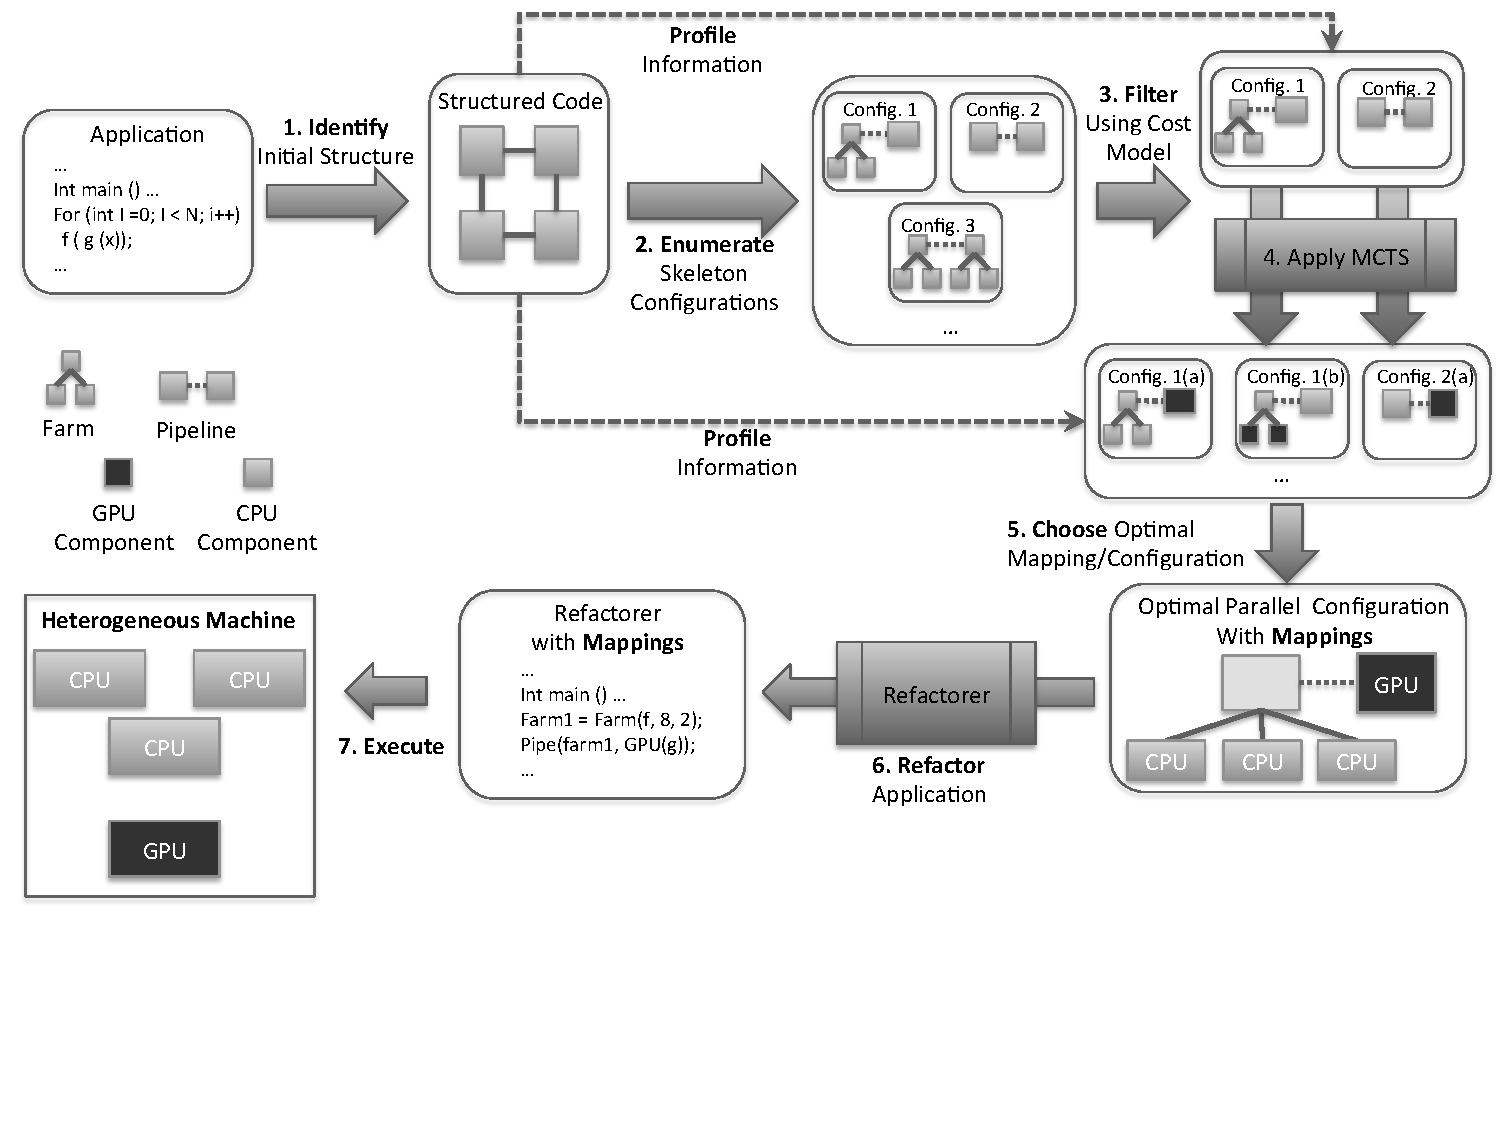
\includegraphics[width=1\linewidth]{figures/methodology.pdf}
\caption{Overview of our technique for programming heterogeneous multi-core systems}
\label{overview}
\end{center}
\end{figure*}

\begin{figure}
\subfigure[Source code for image convolution before refactoring] {
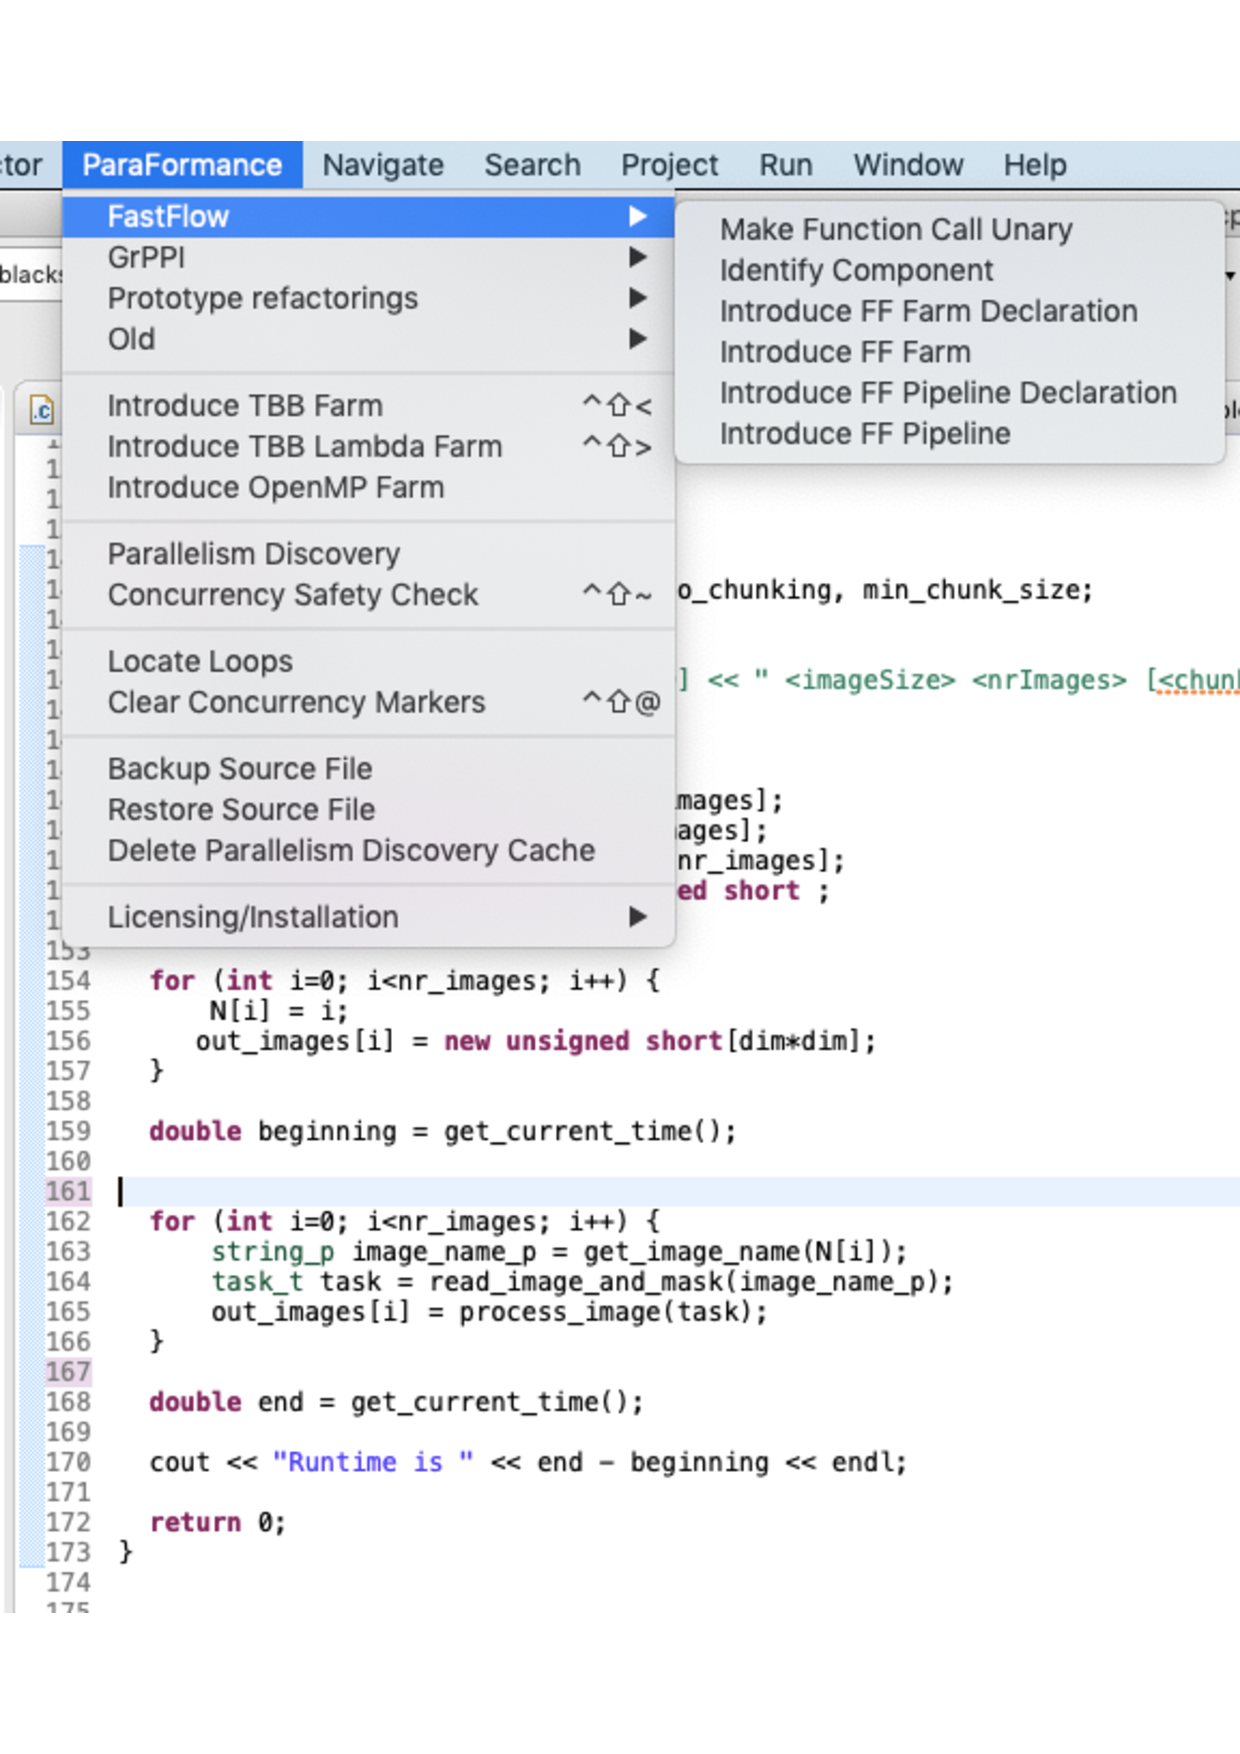
\includegraphics[width=0.42\textwidth]{figures/BeforeRefact.pdf}
\label{fig:beforeRefact}
\vspace{-0.8cm}
}
\hspace{0.05cm}
\subfigure[Source code for image convolution after refactoring] {
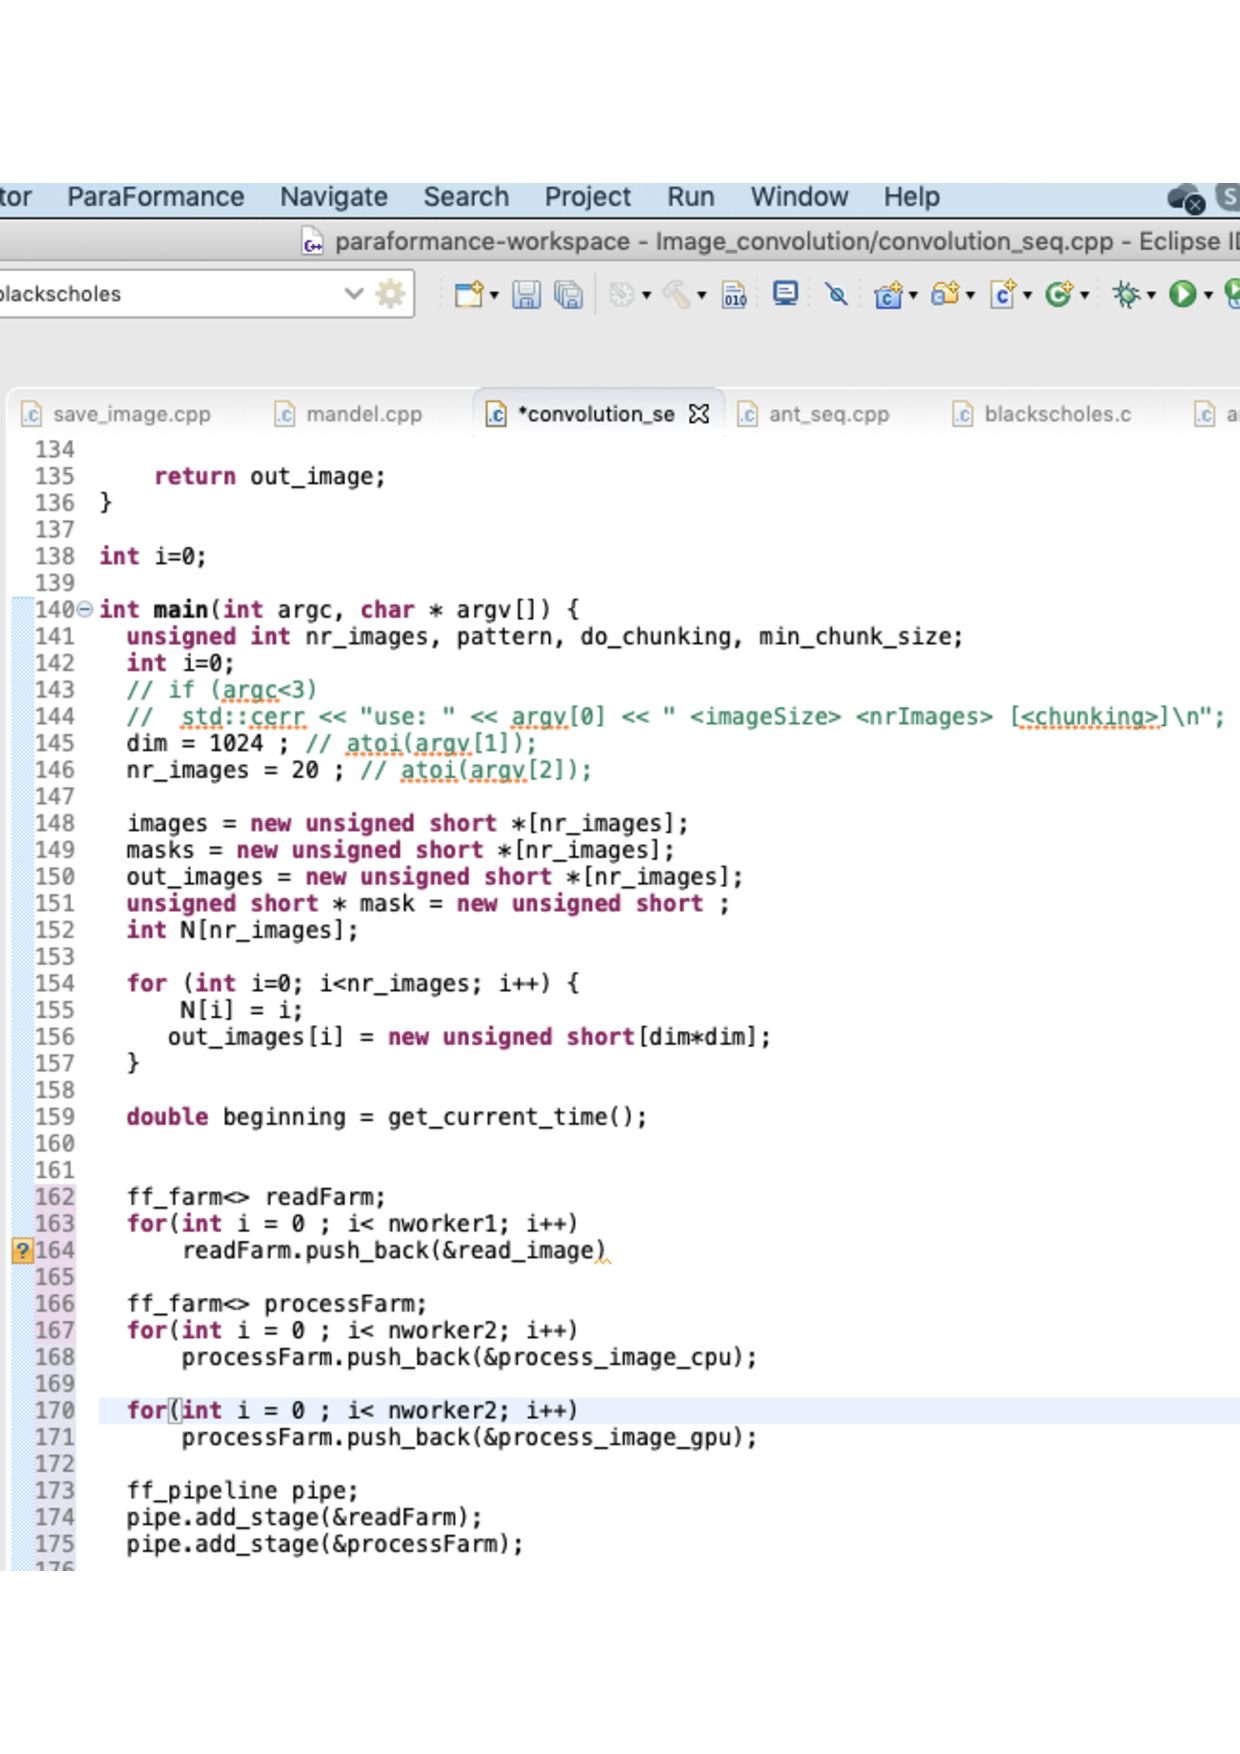
\includegraphics[width=0.44\textwidth]{figures/AfterRefact.pdf}
\label{fig:afterRefact}
\vspace{-0.8cm}
}
\caption{Application of the refactoring tool for introducing parallel patterns in the sequential code}
\label{fig:refactoring}
\end{figure}


% VJ : I would remove this. I think our technology is aimed also at
% good parallel programmers. Besides, we cannot really expect the
% inexperienced parallel programmer to provide us with good
% decomposition of a problem, good CPU and GPU implementations of
% functions etc.
% Our methodology is aimed at inexperienced parallel programmers who lack the experience 
% or expertise in deploying parallelism in their applications, particularly for heterogeneous systems.
\noindent
In this section we introduce a new parallel programming technique aimed at increasing the programmability of heterogeneous 
parallel systems.
Our technique aims to support both the inexperienced parallel programmer with 
little knowledge on parallel programming techniques; and also the experienced parallel programmer, who
seeks to maximize productivity with the appropriate tool support to automate the process. 
Our general technique is shown in Figure \ref{overview} and comprises a number of steps, described below.
\begin{enumerate}
\item \emph{Identifying initial structure.} The programmer starts with a (possibly parallel) application. The first step is to \emph{identify}
 an initial
  skeleton structure in the code corresponding to the skeletons defined in Section~\ref{sec:background}.
  This skeleton structure is recorded in a text file, which encapsulates the basic sequential structure of the
  algorithm, together with its basic units of computation (components) and
  tasks. Components correspond to functions of the source code. 
  We also record what implementations (CPU, GPU or both) exist
  for which components. 
%VJ : Is this automated?

  As a simple example, consider the piece of code in Figure~\ref{fig:beforeRefact} at lines 162---166.
  %following piece of code:
  %\begin{lstlisting}[language=C]
  %for (i=0; i<nrImages; i++) {
   % image = read_image(imageFiles[i]);
%    outImage[i] = process_image(image);
 % }
 %  \end{lstlisting}
  The structure of this code is a composition of two functions,
  \lstinline|read_image| and \lstinline|process_image|, on a stream of
  input files, \lstinline|imageFiles|. Components are the
  functions \lstinline|read_image| and \lstinline|process_image|, and the
  tasks are applications of these functions to the elements of the array,
  \lstinline|imageFiles|. We might only have a CPU implementation of
  the \lstinline|read_image| function, and both CPU and GPU implementations (kernels)
  of the \lstinline|process_image| function.
  Using the notation from Section
  \ref{sec:background}, we can denote this by $r \circ p$, where $r$ is 
  \lstinline{read_image} function, $p$ is
  \lstinline|process_image| function, and $\circ$ is the sequential
  composition. 

%Finally, profiling can give us information that running
 % \lstinline|read_image| for one image on a CPU takes $0.2ms$, running
 % \lstinline|process_image| on a CPU takes $6.6ms$ and running
 % \lstinline|process_image| on a GPU takes $0.08ms$.

\item \emph{Profiling}. After we have identified the skeleton
  structure of the application and its components, we do time
  profiling of the components. That is, we run each available version (CPU or
  GPU) of each component on a sample of input tasks in order to determine
  the average time it takes for each component to process one input
  task. This timing information is used in subsequent  steps of our
  methdology. This step is carried out manually by the programmer, and
  its time complexity depends on the runtime of components for the
  sampled inputs.

  In our working example, using profiling we can obtain information that
  running CPU version of \lstinline|read_image| on one image takes $0.2ms$, running
  CPU version of \lstinline|process_image| on one image takes $6.6ms$ and running
  GPU version of \lstinline|process_image| on one image takes $0.08ms$.

\item \emph{Enumerating Skeleton Configurations}. Given the text file
  with the identified skeleton from the original application, produced
  in step 1, all possible
  equivalent skeleton configurations are automatically generated (up to a given depth of nesting)
  resulting in a number of different possible parallelisations. 
  Given an initial configuration, each composition ($\circ$) can be transformed into a parallel pipeline ($\parallel$) and
  a farm skeleton ($\Delta$) can be introduced for any skeleton configuration\footnote{Since we assume that all functions operate on streams, it is always possible to replace a function with a farm skeleton operating on elements of the input stream in parallel.}. Similarly the inverse of these transformations
  can also be applied; for example, we can transform a parallel
  pipeline into a sequential composition, or eliminate a farm skeleton
  altogether. This step is computationally very cheap and fully automatic.
  %In Figure~\ref{overview}, we refer to step 2 as \emph{enumerating} the skeleton
  %configurations. 

  In our example, in the step 1 we identified the initial structure to be $r \circ p$;  therefore, the possible
  skeleton configurations are $r \circ p$, $\Delta(r \circ p)$, $\Delta(r) \circ
  p$, $r \circ \Delta(p)$, $\Delta(r) \circ \Delta(p)$, $r \parallel
  p$, $\Delta(r) \parallel p$ etc. 
\item \emph{Filtering Using Cost Model}. Using profiling information
  obtained in step 2, the skeleton configurations are \emph{filtered} using a cost model
  to restrict the number of possibilities that need to be considered.
  This allows us to eliminate parallelisations with little or no potential
  speedup at an early stage of development.  In
  Section~\ref{sec:results}, we use a simple high-level cost model to predict
  the best possible run times for each configuration on a given hardware. At
  this stage, exact timing information is not needed, as only very
  poor potential speedups lead to exclusion. Since we use
  simple cost models, this step is computationally very cheap, and
  also fully automatic.

In our example, the cost model may predict that $\Delta(r) \parallel
\Delta(p)$, $\Delta(r) \parallel p$ and $\Delta(r) \circ \Delta(p)$
are the best candidates from all possible factorisations.

\item \emph{Ranking the Configurations and Deriving Mappings}. The remaining configurations are then analysed in more detail,
  deriving optimal (or near-optimal) static mappings for each of them,
  together with the estimated runtime. A static mapping is an
  assignment of number of workers for each farm skeleton in a skeleton
  configuration, together with the type of each worker and each
  pipeline stage (the type can be CPU
  or GPU). Possible types of a farm worker/pipeline stage depend on
  the type of implementation that we have for that kind of
  worker/pipeline stage. This phase, therefore, outputs
  for each configuration, all the missing skeleton parameters. It also 
  gives the ranking of the configurations
  in terms of their expected performance. In this paper, we present
  one possible model for deriving static mappings for a given skeleton
  configuration, based on the Monte Carlo Tree Search (MCTS)
  algorithm~\cite{mc}. This step is fully automatic, and is also
  computationally the most expensive part of the technique. Exactly
  how much time it takes to rank the configurations and derive
  mappings depends mostly on the method used for estimating of the
  application runtime with a particular static mapping. If full simulation is used,
  the cost is very high, whereas if some analytical model is used
  (e.g. some more precise cost model than in step 4), the cost can be
  very low.


%The remaining configurations are then given to the \emph{MCTS} model, together with the profiling
 % information and hardware information. The model outputs, for each
  %configuration, near-optimal skeleton parameters (such as the number of
 % worker thread for each \emph{farm} skeleton in a given
 % configuration), together with the
 % percentages (for each farm) of work that should be done on CPUs and
 % GPUs. This stage, therefore, returns a ranking for the
 % configurations (together with mapping and skeletal parameters),
 % based on the estimated runtime.
%
  In our example, this step can tell us that the best parallelisation on a given
  machine (e.g.\ comprising of 24 CPU cores and 1 GPU) is
  $\Delta(r) \parallel \Delta(p)$, where 15 CPU workers are used for
  $\Delta(r)$ and 9 CPU and 1 GPU workers are used for
  $\Delta(p)$. 
\item \emph{Refactoring the Application}. The programmer then \emph{chooses} one of the parallelisations together with its static mapping
and refactors the original application from Step 1, introducing the
desired skeleton configuration from Step 5 using the \emph{refactoring} tool.
The refactoring tool performs all the required program transformations and condition checking automatically,
introducing the skeleton structure and the parameters from Step
4. This part is semi-automatic and computationally cheap.

Considering the example code from Step 1 and the 
skeleton configuration, $\Delta(r) \parallel \Delta(p)$, the refactoring tool may produce the output as in Figure~\ref{fig:afterRefact},
%
%ollowing:
%  \begin{lstlisting}[language=C]
%  ff_farm<> readFarm;
%  ...
%  for(int i = 0 ; i< nworker1; i++)
%      readFarm.push_back(&read_image)
%  for(int i = 0 ; i< gpu_nworker1; i++)
%      readFarm.push_back(&read_image_gpu)
%  ff_farm<> processFarm;
%  ...
%  for(int i = 0 ; i< nworker2; i++)
%      processFarm.push_back(&read_image)
%  ff_pipeline pipe;
%  pipe.add_stage(&readFarm);
%  pipe.add_stage(&processFarm);
%  ....
%   \end{lstlisting}
where the refactoring tool introduces FastFlow farm and pipeline skeletons (\lstinline{ff_farm} and \lstinline{ff_pipeline})
including the number of CPU and GPU workers for the farm skeletons, \lstinline{readFarm} and \lstinline{processFarm}. These worker parameters are
taken directly from the output of Stage 4. 
\item \emph{Executing the Application}. The refactored program can then be executed on the available heterogeneous hardware, and the 
process can be repeated if necessary. For example, if the programmer decides to port the application to a different
architecture, or if the programmer discovers that an alternative configuration given at Step 5 would be better suited.
\end{enumerate}
%\noindent
%% After the refactoring process, the user is then free to restart the
%% process. 
%%A program may be refactored as many times as necessary.
%%This may be useful if the application is to be ported to a different
%%architecture, for example.
%% with different numbers of CPUs/GPUs, for example. 
%The programmer may restart the process
% with the refactored application, or \emph{undo} any previous refactorings already made, starting 
%with the original sequential program.
%%
%Where a program has already been parallelised, it must first be structured into a component-based program.  Obviously, this might
%involve undoing some design decisions, so that a more structured approach can be used.  However, it might also involve encapsulating
%existing paralellism so that it can be easily reused.  While this is an interesting problem, we will not consider this further in this paper,
%focusing instead on the primary problem of introducing and exploiting parallelism, as a necessary first step.

%We consider a program factorised as a combination of parallel patterns. The factorisation gives rise to a process graph, the leaves of which represent particular units of computation, called functions, which will be allocated, in parallel, to a set of available processors. Processors can be of C (CPU) or G (GPU) type. Decisions must be made on how much computational resource and of which type (C or G) will be allocated to the parallel computation of each function. The Static Mapping Problem is to determine a fixed allocation of processing resource to functions to maximise the throughput of the parallel program.

%The process tree along with a policy defines a process graph which shows the sequence of processing starting from input running through a set of patterns. An input packet is passed to the first pattern. It passes through a series of structural boxes ending at a leaf which is the function for which it is the input. That function is executed on a processor selected by the policy. The outputs are then passed through the structure to the next function leaf and so on. This happens in parallel so that many sequences of processing are being executed in parallel.


%Our aim is to make available, in design time, a means of identifying an optimal static mapping with regard to throughput. Given the above assumptions, any parallel program may be characterised by its pattern tree and the set of distributions of function timings. For a fixed tree depth, it is possible to generate all possible abstract factorisations raising the possibility of similarity matching between parallel programs by structure and function profiles. Thus learning about optimal static mappings can potentially be transferred from stored calculations to new programs at the design stage.  Optimisation can be regarded as a search through possible static mappings with the aim of maximising throughput. 

\section{Deriving Mappings using Monte Carlo Tree Search}
\noindent
In this section, we describe a model that we use to derive, for a
given skeletal configuration, a good  static mapping of its components to
the available hardware. A static mapping in our case corresponds to a
particular choice of values for the parameters of skeletons, i.e.\ the number of workers in
each farm, the type (CPU or GPU) of each worker in each farm and each stage of each pipeline. 
The quality of a mapping is derived from a specific evaluation function $Q$, being a combination of the runtime and the resource utilisation. 

Our model accepts as an input a skeletal configuration and
the timings for its components (derived from profiling both for CPU and
GPU versions, if the GPU version of a component is available). As an
output, it produces a candidate static mapping  and the corresponding estimated runtime of the skeletal
configuration. Since considering all possible static mappings for a given
skeletal configuration may be computationally intractable, an optimisation method is used. Here, we use the Monte Carlo Tree Search (MCTS) approach, well known for generating and
evaluating large game trees in Game theory. In our case,   the nodes of the
generated tree correspond to partial mappings (with some of the
skeleton parameters chosen) and the leaves of the tree correspond to
complete mappings. The children of a node represent different possible
assignments of a yet unassigned skeleton parameter.

The MCTS approach starts from a tree that consists only of a
single 
root node (i.e.\ a static mapping where no
parameters are chosen). It proceeds by repeating the following three steps: 
\begin{enumerate}
\item \emph{Expansion step} -- A node (corresponding to
  a partial static mapping) is selected, and one of its children is
  added to the tree. This is equivalent to assigning a value to one previously unassigned
  parameter;
\item \emph{Selection step} -- Starting from the newly added node, a
  complete static mapping is generated by randomly assigning the
  remaining unassigned parameters. The resulting static mapping is evaluated based on the 
  evaluation function, $Q$, yielding the valuation $v$;
\item \emph{Propagation step} -- The valuation, $v$, is propagated back
  to the node added in step $1$. 
\end{enumerate}

\noindent
Steps 2 and 3 are repeated a fixed number of times, attaining a reliable evaluation of the partial mapping in step 1 by evaluating a fixed number of random complete mappings that correspond to it. In this way, we  avoid the exhaustive search of all complete mappings corresponding to that partial one. Then, step 1 is repeated, adding a new value to the partial mapping.
Finally, the overall best complete mapping (a leaf of the tree) is
selected. 
%This branch corresponds to the static mapping that is returned by the model.


% VJ : Something is obviously missing here

% A challenge is then to
%efficiently gain sufficient information from the simulation 
% to discriminate between mappings with a level of confidence.
% In order to customise the MCTS for our static mapping problem,
% we model the allocation as a sequence of decisions that determines the quantity of 
% the available remaining resource that should be allocated to a particular component. At each decision point, some resources will be allocated, 
% limiting the resources available to, as yet, unallocated components. We reach a leaf of the tree precisely when all components have been allocated 
% an amount and type of resource (which in pathological cases may be zero). At this point the mapping can be evaluated by simulation. We will apply 
% MCTS to search for an optimal path through this decision tree. The order of decisions is determined by the queue bottleneck. So the first 
% children of the tree will be the queue with the least throughput, the second level will be the second least throughput queue, and so on. This 
% creates a decision tree that is perfectly suitable for breadth-first search algorithms.

%Therefore, a given static mapping allows a simulation of the computation as random-walks where, at each step, a decision is made to allocate a 
%particular package of processing to a particular processor. The walk is biased by the parameters of the static mapping. At the end of the walk, 
%an evaluation function is calculated to measure the performance distributions on the assigned processors.

%The evaluation function is based on the throughput of the system which we denote by $T$.
%There are two balancing factors relating to the number 
%of resources allocated to the components of the system.
%$SD_U$ is the standard deviation of  the utilisation of all components in the system:

The function that we use to evaluate how good static
mappings are is based on the estimation of the runtime for that static
mapping that we obtain using simulations, and the utilisation of the
system. The function is

% VJ : What are queues, components? I don't get this
% CWG : I dont get it either. This is super confusing, especially due to variable "overloading". I will try to rewrite

$$Q(M) = S(M) - (\delta_U(M) + \delta_Q(M)),$$
where $S(M)$ is the estimated throughput of the whole system (i.e.\
the number of tasks per unit of time that get processed, obtained using profiling)
$\delta_U(M)$ is the standard deviation of the utilisation of
components (where the utilisation of a component is the ratio between the time the component spends
executing tasks and the total execution time of the application) and $\delta_Q(M)$ is the standard deviation of
the utilisation of the connecting queues between the components (where
the utilisation of a queue is the ratio between the time where at least
one task was in the queue and the total execution time) in the skeleton. Using this function, $Q(M)$, rather than using
just the throughput, $S(M)$, as an evaluation function, discourages the allocating of more resources to the skeleton configuration, if
it only results in marginally improved runtime, which may be important
in settings where resources are paid for (e.g.\ clouds).

\subsection{Adaptation of the MCTS Technique to the Static Mapping
  Problem}

\noindent It is well known that the MCTS techinque is most often used
to find a single best move at the root of the game tree. In our
adaptation of the technique to the static mapping problem, the best
move at the root of the tree represent assignments of all the
parameters to all the components of the application. \textbf{ToDo: }
\emph{This needs to be thought over, because in the text above, we say the
opposite - that the root of the tree represents the mapping where no
parameters have been assigned.}

\noindent
\paragraph{Suitability of Using MCTS to Derive Static Mappings} The
main target for the MCTS-based approach for deriving static mappings
are computationally-heavy parallel applications that contain nested
parallelism in the form of farms and pipelines. Such applications
might take hours or even days to execute and may need to be executed
repeatedly, so the effort required by the MCTS model to derive
near-optimal mappings is well justified by savings in time and energy
of the optimised parallel applications. In addition, solution space,
even when the degree of nesting of skeletons is relatively small, is
sufficiently large to justify the use of MCTS. For example, for the
Image Convolution problem considered in Section~\ref{sec:imageConv},
with the depth of skeleton nesting of 2, the Table~\ref{tab:conv}
gives an example sizes of solution space for different hardware
configurations and the estimated time needed to evaluate all of them
using full profiling (which is the only way to give the accurate
estimation of the execution time). From the table, we can see that for
even modestly-sized parallel systems, the time to evaluate all
parameters would be hundreds of days order of magnitude. Since
parallel systems are becoming larger and larger, with more CPU cores
and more GPU devices being available in a single shared-memory system,
the problem will only become more time-consuming.

\begin{table}
  \begin{tabular}{|c|c|c|c|c|}
    \hline \hline
    \textbf{CPU Cores} & \textbf{GPUs} & \textbf{App Components} &
    \textbf{Sol. Size} & \textbf{Time for Eval.} \\
    \hline
    16 & 1 & 4 & 1240 & $>$86400s \\ \hline
    24 & 2 & 4 &6624 & $>$604800s \\ \hline
    64 & 2 & 4 & 129204 & $>$36288000s \\
    \hline \hline
  \end{tabular}
  \caption{Solution space and time needed for its full evaluation for
  Image Convolution on different hardware configurations.}
  \label{tab:conv}
\end{table}

\paragraph{MCTS Parameters} The selection strategy that we use is the \emph{Upper Confidence bounds applied to Trees} (UCT)~\cite{kocsis2006improved}.
The formula for UCT is

$$UCT= \overline{X_j} + 2C_P\sqrt{\frac{2\ln n}{n_j}},$$

\noindent
where $n$ is the number of times the current node has been visited; $n_j$ is the number of times the child, $j$, has been visited;
$C_P>0$ is a constant value; and, $\overline{X_j}$ is the average
reward value given to child node, $j$. The experiments showed that the
value of around 1/5th of the average throughput for $C_P$ gives the
best results, being a good tradeoff between reducing the search space
and making sure we do not get stuck in the local optimum. As for the back-propagation
policy, we considered two policies - \emph{Max} policy, where the
maximal reward of all the children is propagated to their parent, and
the \emph{Average} policy, where the average reward of all the
children is propagated to their parent. The experiments showed that
the \emph{Average} policy works better, being less greedy. For more
details, see~\cite{cec2013}.



%$SD_U = \sqrt{\frac{\Sigma_{N}(U_{w_i}-U{w_{m}})^2}{N}}$

%Here, $N$ is total number of component sin the system, $U_{w_i}$ is the utilisation of the component, and $w_i$ and $U_{w_{m}}$ are the average utilisation values of all components in the system. 
%Adjusting the reward for this factor discourages the allocation of additional resources to components of queues  which are no longer bottlenecks.

%$SD_Q$ is the standard deviation of all queues in the system, defined:

%$SD_Q = \sqrt{\frac{\Sigma_{L}(T_{Q_i}-T_{Q_{m}})^2}{L}}$

% Here, $L$ is the total number of queues in the system, $T_{Q_i}$ is the throughput of the $Q_i$, and $T_{Q_{m}}$ is the average
% value of the throughput of all queues in the system. 
% Adjusting the reward for this factor discourages the allocation of additional resources to the components of a queue when they are no longer bottlenecks for that queue.%this may need further explanation

% Adding these two factors allows the algorithm to find the optimum 
% number of resources for the system, especially when the resources are, for example, on ``the cloud" where resources are typically expensive. Adding these two 
% penalty function can reduce the resource cost.

% Considering all these factors, the evaluation function $Q(v)$ for each selected path $v$ is defined:


% $Q(v) = T - (SD_{U} + SD_{Q})$ 
% 
%\section{Refactoring}
%%[01/02/2013 15:57:38] Vladimir Janjic: skeleton rewrite rules are fine
%%[01/02/2013 15:57:46] Vladimir Janjic: but they are abstract and not very usable, right?
%%[01/02/2013 15:57:55] Vladimir Janjic: in order to apply them in a given language
%%[01/02/2013 15:58:01] Vladimir Janjic: you still need to do all work yourself
%%[01/02/2013 15:58:09] Vladimir Janjic: i.e. check that rules can be applied
%%[01/02/2013 15:58:17] Vladimir Janjic: check that semantics is preserved
%%[01/02/2013 15:58:22] Vladimir Janjic: and all that
%
%\noindent
%%% Intro/conclusion. KH
%% We describe the refactorings here in terms of C++, but with a FastFlow
%% skeleton approach, to demonstrate the principles of our methodology.  The
%% refactorings could easily be demonstrated for other skeleton approaches
%% and frameworks, and not are not limited to C++.  
%Our refactoring
%prototype is implemented in Eclipse, % a popular C++ IDE, 
%under the CDT plugin. The programmer is presented with a menu of possible refactorings to
%apply.  The decision to apply a refactoring and identify a possible
%skeleton to introduce is made by the programmer. Once a decision
%has been made, any required transformation and mapping is performed automatically. In this way, we can rely on programmers making informed
%decisions about which refactorings to apply, but do not rely on them % who may not have the
%necessarily having expertise with parallelism or skeletons.  Figure~\ref{eclipse}
%shows a sample screenshot of our refactoring tool, where the programmer is
%presented with a menu of possible parallel refactorings to apply, such as
%\emph{Introduce Farm} and \emph{Introduce Pipeline}, described below: %, which we discuss in more detail here.
%
%\begin{itemize}
%\item \textbf{Introduce Pipeline}.
%% Here we define the \emph{Introduce Pipeline Refactoring}. 
%For this refactoring, the programmer must select a \texttt{for} loop, e.g.,
%the \texttt{for} loop that is shown in the first column of Figure \ref{refacex}.
%The second column in the figure shows the effect after refactoring. % , which is a an \emph{automatic} transformation. 
%% In the second column of the figure, 
%Here, the original \texttt{for} loop has been re-written into a
%\texttt{StreamGen} stage. This is a C++ class instance that models the
%streaming input behaviour to the pipeline.  The refactoring is not
%limited to only C style arrays, however, as C++ STL data structures may
%also be considered, such as \texttt{std:vector< >} objects.  In the
%second column, an instance of a FastFlow \emph{Pipe}line skeleton has
%been introduced, named \texttt{pipe}.  The first stage, a function,
%\texttt{ff\_pipe\_first\_stage}, is added as a pipeline stage; the second
%stage, \texttt{CPU\_Stage}, is added as the final stage.  Finally, the
%pipeline waits for the result of the computation, using a \texttt{run()}
%method call.  The dependency between the output of
%\texttt{ff\_pipe\_first\_stage} and the input of \texttt{CPU\_Stage} is
%detected automatically. % by the refactoring.
%
%\item \textbf{Introduce Farm}.
%% Here we introduce the \emph{Introduce Farm Refactoring}, as demonstrated 
%%This is shown in the third column of Figure \ref{refacex}.
%  Here the refactoring has two variants: farming a \emph{Pipe}line stage;
%  or, alternatively, introducing a new \emph{Farm}.  Farming a pipeline
%  stage is the simplest of the two variants.  The middle column of
%  Figure~\ref{refacex} shows a stage of an already defined FastFlow
%  \emph{Pipe}line skeleton that the programmer has highlighted.  The
%  result of the refactoring is shown in the right column: the \emph{Pipe}
%  skeleton has been modified to replace the selected stage---here, the
%  function \texttt{ff\_pipe\_first\_stage}---with a FastFlow \emph{Farm},
%  called \texttt{global\_farm}. All other stages in the \emph{Pipe}line
%  are preserved. The refactoring requires that \texttt{nworkers} (the
%  number of \emph{Farm} workers) to be either previously defined, or given as an
%  explicit argument to the refactoring.
%\end{itemize}
%Each of the introduction refactorings has a corresponding inverse:  \emph{Farm Elimination} inverts \emph{Introduce Farm};
% \emph{Pipeline Elimination} inverts \emph{Introduce Pipeline}. This allows any
%combination of rules to be inverted, or undone, as part of a 
%parallel refactoring process.  The refactorings are also fully nest-able,
%allowing, for example, a farm, such as $\Delta(f1 \circ f2)$ (a task farm
%where the worker is a function composition of two components, \emph{f1}
%and \emph{f2}), to be refactored into $\Delta(f1 \parallel f2)$.
%
%%\subsection{Tuning Parallelism}
%%\begin{itemize}
%%\item \textbf{Skeleton Tree to Skeleton Tree}
%%\item \textbf{Chunking}
%%\item \textbf{GPU Variants}
%%\end{itemize}


%\section{Background} \label{sec:background}


%\subsection{Skeleton Cost Models}  \label{sec:costmodels}
%\noindent
%In this section we give a corresponding high-level cost model for each
%skeleton in Section \ref{sec:skeletons}, derived after those presented in  \cite{DBLP:books/daglib/0098705,DBLP:conf/europar/CaromelL07}. 
%These cost models estimate the runtime of a particular skeleton
%configuration on a sequence of inputs, on a particular hardware.
%The cost models that we consider here are intentionally high-level and simple, abstracting over
%many language- and architecture-specific details. Their only purpose is to give us
%a very rough performance estimate for a skeletal configuration.
%If desired, more complex models could be used to yield more accurate
%predictions for a specific architecture. 
%%without changing the general methodology.
%
%\noindent
%Function \emph{Comp}osition ($\circ$) can be costed trivially:
%$$T_{\circ}((f_1, \dots, f_n), (x_1, \dots, x_m))  = m
%\cdot \sum_{i=1}^{n}{T(f_i)}$$
%where $T(f_i)$ represents the estimated runtime of function $f_i$ for
%one input. This formula assumes that the functions $f_1, \dots, f_n$
%are regular, i.e.\  that the time it takes to compute $f_i(x)$ is the
%same for every $x \in \{x_1, \dots, x_m\}$. 
%
%
%A cost model for the pipeline is:
%$$T_{\parallel}((f_1, \dots, f_n), (x_1, \dots,
%x_m)) =$$ $$=\sum_{i=1}^n T(f_i) + (m-n) \cdot \max_{i \in \{1,n\}} T(f_i).$$
%This defines the cost of a steady-state pipeline in terms of the
%initial cost of filling the pipeline with $n$ values, plus the cost of the most expensive
%pipeline stage for the remaining $m-n$ values. As in the previous
%case, this formula also assumes regularity of all functions $f_1,
%\dots, f_n$.
%
%The cost model for the farm skeleton is
%$$T_{\Delta}(f, (x_1,\dots,x_m)) = $$ $$=T(f) \cdot \lceil \frac{m}{\min\{n_p,n_w\}} \rceil + (D + G) * \min\{n_p, m\},$$
%where $n_p$ is the number of independent cores in the system, $n_w$ is the
%number of worker threads, $D$ is the cost of distributing the input
%values to the worker threads and $G$ is the cost of gathering the
%results from the workers. In our case
%$$D = D(n_w,m) = n_w \cdot S + n_w \cdot (I + C(\frac{m}{n_w}))$$
%$$G = G(n_w,m) = n_w \cdot (I + C(\frac{m}{n_w})),$$ 
%where $S$ is the cost of spawning the worker thread, $I$ is the cost
%of initialising the worker thread and $C(n)$ is the
%cost of copying $n$ items of data between two threads



%\subsection{Refactoring}
%Refactoring is the process of changing the internal structure of a program, while preserving its behaviour \cbcomment{mention that parallelisation refactorings do change bevahiour, it's functional correctness that is preseved}. The term refactoring was first introduced by Opdyke in his PhD thesis in 1992 \cite{opdyke} and the concept goes back to the fold/unfold system proposed by Darlington and Burstall in 1977 \cite{darlington77}. The key aspect of refactoring is the focus on purely structural changes rather than changes in program functionality.
%Unlike automatic program compilation and optimization, refactoring emphases the software development cycle, principally by:
%improving the design of software; making software easier to understand; encouraging code reuse; increasing productivity; and increasing programmability.
%
%Automated parallelisation techniques, which work only for a very limited set of cases under extreme conditions are not simply tractable nor general.
%In this paper, we introduce a new approach for solving the parallelism crisis: by using advanced refactoring techniques

% VJ : Not needed any more
% \subsection{Pattern-Trees}
% \noindent
% In the methodology presented in Section \ref{sec:methodology}, we make
% use of a concept of a \emph{pattern tree}, which models a high-level
% structure of the application. 
% Pattern tree is used to determine different possible factorisations
% (skeletal configurations) of the pattern, to be passed
% to the MCTS stage, which then determines the mapping parameters, such as the number of workers, $nw$, and %
% which components should execute on the CPU or GPU. 
% The pattern-tree encapsulates the minimal information from each skeleton in order
% to express the abstract structure of the application.
% Therefore our pattern tree is void
% of the input stream to the skeleton, together with any extra parameters such as the number of workers.
% In our pattern-tree notation,
% we denote \emph{Farm} as $\Delta(f)$; \emph{Pipe} as $f1 \parallel f2$; and \emph{Comp} as $f1 \circ f2$,
% where $f1$ and $f2$ are also possible pattern-trees or computations (either CPU or GPU).

%\begin{figure*}[t]
%\begin{center}
%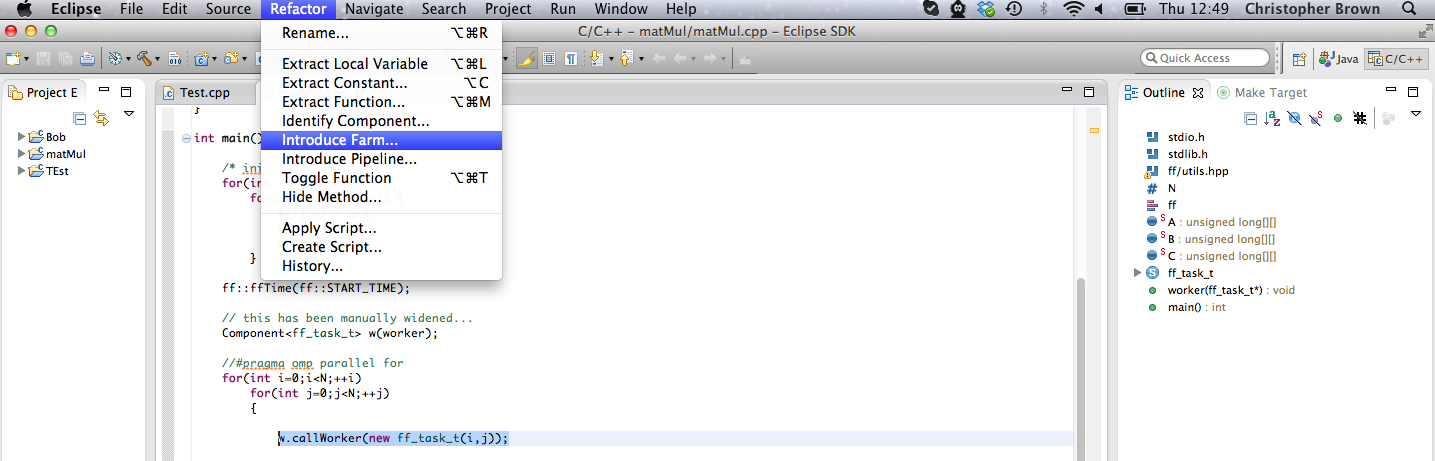
\includegraphics[width=0.95\linewidth]{figures/eclipse.png}
%\caption{C++ Parallel Refactoring Tool in Eclipse}
%\label{eclipse}
%\end{center}
%\end{figure*}
%
%\begin{figure*}
%\begin{center}
%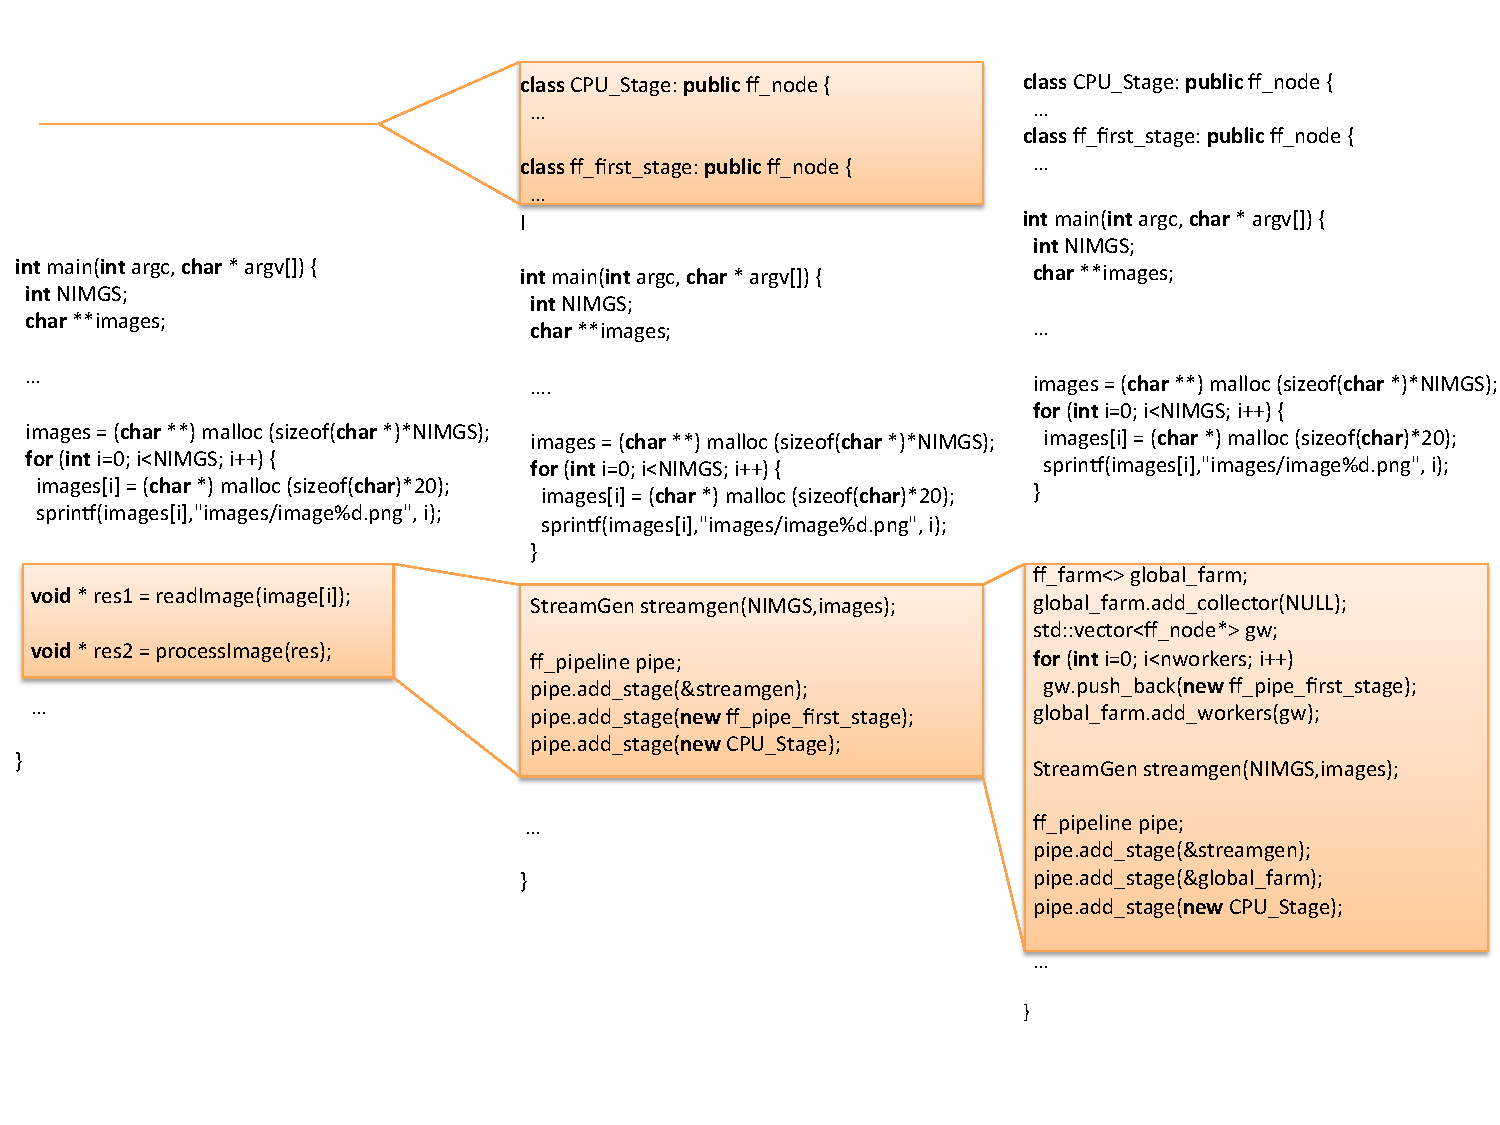
\includegraphics[width=0.95\linewidth]{figures/refactoring.pdf}
%%\begin{minipage}{0.33\linewidth}
%%\begin{scriptsize}
%%\begin{lstlisting}[language=C++, caption=Sequential Version]
%%struct Image 
%%
%%Image* georef(Image* image) {
%%  ...
%%
%%Image* denoise(Image* image) {
%%  ...
%%
%%int main(int argc, char* argv[]) {
%%  ...
%%  // the following part of code is 
%%  // highlighted by the programmer
%%  // in the refactoring tool
%%  for(int i=0; i < N; i++) {
%%     result1 = georef(inpt[i]); 
%%     results[i] = denoise(result1);
%%  }
%%  // do something using the results 
%%  // array
%%}
%%\end{lstlisting}
%%\end{scriptsize}
%%\end{minipage}%
%%%\hfill\vrule\hfill
%%\begin{minipage}{0.33\linewidth}
%%\begin{scriptsize}
%%\begin{lstlisting}[language=c++, caption=Introduce Pipeline]
%%struct Image 
%%
%%Image* georef(Image* image) {
%%  ...
%%
%%Image* denoise(Image* image) {
%%  ...
%%
%%int main(int argc, char* argv[]) {
%%  ...
%% ff_pipeline pipe;
%% StreamGen<Image> streamgen(NIMGS, 
%%                            images);
%% GenNode<Image> stage1(georef);
%% GenNode<Image> stage2(denoise, 
%%                       results);
%% pipe.addStage(&streamgen);
%% pipe.addStage(&stage1);
%% pipe.addStage(&stage2);
%% results = pipe.run_and_wait_end();
%% 
%% // do something using the results 
%% // array
%% 
%%}
%%\end{lstlisting}
%%\end{scriptsize}
%%\end{minipage}%
%%\begin{minipage}{0.33\linewidth}
%%\begin{scriptsize}
%%\begin{lstlisting}[language=c++, caption=Introduce Farm]
%%struct Image 
%%
%%Image* georef(Image* image) {
%%  ...
%%
%%Image* denoise(Image* image) {
%%  ...
%%
%%int main(int argc, char* argv[]) {
%%  ...
%% ff_pipeline pipe;
%% StreamGen<Image> streamgen(NIMGS, 
%%                            images);
%% GenNode<Image> stage1(georef);
%% GenNode<Image> stage2(denoise, 
%%                       results);
%% pipe.addStage(&streamgen);
%% 
%% ff_farm<> geoFarm;
%%    std::vector<ff_node*> v;
%%    for(int i=0;i<NW;++i) v.push_back(
%%                 new GeoRef);
%%    geoFarm.add_workers(v)
%%
%%    geoFarm.add_collector(NULL); 
%% 
%% pipe.addStage(&stage1);
%% pipe.addStage(&stage2);
%% results = pipe.run_and_wait_end();
%% 
%% // do something using the results 
%% // array
%%}
%%\end{lstlisting}
%%\end{scriptsize}
%%\end{minipage}
%\caption{The Evolution of a Skeleton Program Using Refactoring: Introduce a Pipeline Skeleton and then Introduce a Farm Skeleton for a Convolution Algorithm.}
%\label{refacex}
%\end{center}
%\end{figure*}
% In~\cite{mpdp}, a heterogeneous skeletal framework was added to FastFlow which allows the programmer
% to incorporate the GPU code. 
% It should arguably be particularly useful in the
% context of heterogeneous multi-core CPU and GPU platforms.
% In~\cite{mpdp}, a heterogeneous skeletal framework was added to FastFlow which allows the programmer
% to incorporate the GPU code. 
% However the number of CPU/GPU workers allocated to each component remains a choice which has to be configured manually by 
% the programmer.

% VJ : eh?
% In~\cite{collinsoptimization} an empirical exploration of the optimisation space under the FastFlow framework was conducted. It was demonstrated 
% that a 70\% improvement for a particular FastFlow application was achieved by tuning the number of component instances and the connected 
% queue size of each component. This further motivates the need for auto-tuning.
\section{Case Studies} \label{sec:results}

\noindent
In this section we demonstrate our technique on three
realistic case studies. For each application, we show different steps of
its parallelisation: 
\begin{enumerate}
\item starting from a sequential version, we
show a number of different possible skeleton configurations; 
\item if the number of skeleton configurations is
  large, we pre-filter these configurations using a cost model
described in~\cite{hlpp} to eliminate weak configurations
(i.e.\ those that would only give small speedups); 
\item we apply MCTS to the remaining configurations to discover the estimated optimal 
static mappings for each of them, and to find out which configuration
(with its corresponding static mapping) delivers the best speedup;
\item  finally, we evaluate the static mappings for each skeleton
configuration resulting from Step 3, in order to
verify the accuracy of the result returned by MCTS.
\end{enumerate} 

\noindent
We consider applications that belong to different domains, showing the
generality of our parallelisation technique. The applications we consider are
Image Convolution, Ant Colony
Optimisation and Molecular Dynamics. The evaluations of the skeleton
configurations in Step 4 are performed on a machine comprising 2x2.4Ghz 12-core 
AMD Opteron 6176 CPUs, coupled with an NVidia Tesla C2050 graphic card
with 448 CUDA cores running at 1.16GHz, running CentOS Linux. The speedups reported in the figures are
averages over 5 independent runs.


\subsection{Image Convolution}
\label{sec:imageConv}
\noindent
Image convolution is a technique widely used in image processing applications such as blurring, smoothing
or edge detection. 
The basic structure of the convolution algorithm is a two-stage function composition, $ r \circ p $.
$r$ is a stage that reads in an image from a file and $p$ is a stage
that processes the image by applying a filter. This
convolution process is typically applied to a stream of input images,
where the output is also a stream.
For each pixel of the input image, the filtering stage consists of computing the scalar product of the
filter and the window surrounding the pixel:
\begin{multline}
\label{eqn:01}
output\_pixel(i,j)=\sum_{m}\sum_{n} input\_pixel(i-n,j-m)\times\\
filter\_weight(n,m){}
\end{multline}
%In order to develop the convolution problem for a
%Heterogeneous system, using FastFlow, we created a subclass \texttt{ff\_node} to implement $r$ (which cannot be executed on a GPU).
%To implement the second stage, $p$, to execute on a GPU, we created a subclass, \texttt{ff\_gpu\_solve} which is derived from
%\texttt{ff\_oclNode}.

\subsubsection{Configurations and Cost-Model Filtering}
\begin{figure}[t]
\begin{center}
\begin{tabular}{| l | l |}
\hline
 Configuration & Est. runtime \tabularnewline
\hline
\hline
$ r \circ p $ & 5.60  \tabularnewline
\hline
$r \parallel p$ & 3.88 \tabularnewline
\hline
$ \mathbf{\Delta(r) \parallel p}$ & \textbf{1.60} \tabularnewline
\hline
$ r \parallel \Delta(p)$ & 4.00 \tabularnewline
\hline
$\mathbf{\Delta(r) \parallel \Delta(p)}$ & \textbf{0.40}  \tabularnewline
\hline
$\mathbf{\Delta(r \parallel p)}$ & \textbf{0.56}  \tabularnewline
\hline
$\Delta(r \circ p)$ & 5.60  \tabularnewline
\hline
$\Delta(r) \circ \Delta(p)$ & 2.00  \tabularnewline
\hline
$\Delta(r) \circ p$ & 2.00 \tabularnewline
\hline
$r \circ \Delta(p)$ & 5.60 \tabularnewline
\hline
\end{tabular}
\caption{Skeleton configurations and their cost-predicted runtimes for
  the Image Convolution}
\label{fig:configsConvolution}
\end{center}
\end{figure}
\noindent

Figure \ref{fig:configsConvolution}  shows all possible
skeleton configurations for the image convolution, up to a nesting depth of two. The first column shows the skeleton configuration, using the
notation introduced in \ref{sec:background}, and the second column shows the
cost-estimated minimal runtime for that configuration. 
The minimal runtime is taken over all possible combinations of workers in each skeleton farm.
Using profiling, we obtained
sequential timings for functions $r$ and $p$ on one $4096*4096$ image, where
$T(r_{CPU})=0.2ms$, $T(p_{CPU})=6.6ms$, $T(p_{GPU})=0.08s$.
In Figure~\ref{fig:configsConvolution}, the bold results are the three best configurations we have selected for further
processing using the MCTS model.


%\subsection{Configurations and Cost-Model Filtering}
% \label{sec:configurations}

%\begin{figure}
%\begin{center}
%\begin{tabular}{| l | l | l |}
%\hline
% Configuration & CPU Time & CPU+GPU Time \tabularnewline
%\hline
%\hline
%$ r \circ p $ & 136.00 & 5.60  \tabularnewline
%\hline
%$r \parallel p$ & 125.60 & 3.88 \tabularnewline
%\hline
%$ \mathbf{\Delta(r) \parallel p}$ & \textbf{132.00} & \textbf{1.60} \tabularnewline
%hline
%$ r \parallel \Delta(p)$ & 13.20 & 4.00 \tabularnewline
%hline
%$\mathbf{\Delta(r) \parallel \Delta(p)}$ & \textbf{13.20} & \textbf{0.40}  \tabularnewline
%hline
%$\mathbf{\Delta(r \parallel p)}$ & \textbf{13.60} & \textbf{0.56}  \tabularnewline
%\hline
%$\Delta(r \circ p)$ & 13.60 & 5.60  \tabularnewline
%\hline
%$\Delta(r) \circ \Delta(p)$ & 13.60 & 2.00  \tabularnewline
%hline
%$\Delta(r) \circ p$ & 132.40 & 2.00 \tabularnewline
%\hline
%$r \circ \Delta(p)$ & 17.20 & 5.60 \tabularnewline
%\hline
%\end{tabular}
%\caption{Cost-predicted runtimes (in milliseconds) for both CPU and
 % CPU+GPU versions of the considered skeleton configurations for image convolution}
%\label{fig:configsConvolution}
%\end{center}
%\end{figure}
%\noindent

%The figure also shows the predicted runtime for each
%configuration, as estimated by our cost model for our 24-core testbed
%machine. The estimations are based on the following profiling  
%For our example, we consider
%introducing a \emph{Farm} ($\Delta$) in both stages of the
%\emph{Pipe}line ($\parallel$), this is justified by the fact that it is
%plausible to read in multiple images from a database at the same time,
%for example, when processing multiple medical images, or when reading
%from multiple CCTV videos simultaneously~\cite{ediPhd}.  In
%Figure~\ref{fig:configs}, we show the different possible pattern-tree
%configurations for the convolution algorithm, up to a nesting depth of 2.
%We also show the predicted runtimes of each configuration based on the
%results of our high-level cost models for both a CPU and GPU. The times
%shown are the best predictions for our 24-core testbed machine, based on the
%following settings (obtained by profiling the application):
%$L=20$, $r = 0.2ms $, $p_{CPU} = 6.6ms$, $r_{GPU} = 0.08ms$. Using these
%profiling results, we can instantiate the cost models from the
%previous section, using profiling, to give a minimal
%$T_{gather}=0.001ms$ and $T_{dist}=0.001ms$.  The high-level cost models
%give us an estimated minimal runtime for each configuration, which we can
%use to filter out weak candidates. Based on the cost model predictions,
%we isolate the top three configurations as candidates for our MCTS model.
%These candidates are shown in bold in Figure~\ref{fig:configs}.

\subsubsection{Optimal Static Mappings Determined by MCTS}

\begin{figure}
\begin{center}
\begin{tabular}{| c | c | c | c |}
\hline
&  $ \Delta(r) \parallel \Delta(p) $ &  $\Delta(r) \parallel p$ & $\Delta(r \parallel p)$ \tabularnewline
\hline
\hline
\begin{tabular}{c}
Mapping \\ (C,G)
\end{tabular}  & $(6,0) \parallel (0,3)$ & $(4,0) \parallel (0,1)$ & $(5,5)$ \tabularnewline
\hline
\end{tabular}
\caption{MCTS predicted optimal mappings for three
  configurations of the Image Convolution example. $(C,G)$ denotes the number of CPU and GPU workers
  for a farm.}
\label{fig:predicts}
\end{center}
\end{figure}

Figure \ref{fig:predicts} shows the output of MCTS for
the three best skeleton configurations for image convolution. The
figure shows, for each farm in each configuration, the estimated optimal number of CPU 
and GPU workers, denoted by a pair $(C,G)$ where $C$ is the number of
CPU workers and $G$ is the number of GPU workers.

\subsubsection{Evaluation of Skeleton Configurations}

\begin{figure}
\begin{center}
\begin{tikzpicture}
\begin{axis}[
  mark size=0.6mm,
  cycle list={
    {blue,mark=star},
    {red,mark=diamond},
    {brown!60!black,mark=triangle},
    {blue,dashed,mark=star},
    {red,dashed,mark=diamond},
    {brown!60!black,dashed,mark=triangle},
  },
  legend style={
    font=\small,
    cells={anchor=west},
  },
  legend pos= north east,
  enlargelimits,
  xtick={1,4,8,12,16},
  ytick={1,5,10,15,20,25,30,35,40},
  %ymin=1,
  ymax=40,
  xlabel=No. CPU workers in $\Delta(r)$,
  ylabel=Speedup,
  title=Speedups for $\Delta(r) \parallel p$
  ]
\addplot table[x index=0,y index=1] {results/version3.txt};
%\addlegendentry{ $GPU = 1$}
%\addplot table[x index=0,y index=3] {Actual2.txt};
%\addlegendentry{Farm with Chunk 16}
%\addplot table[x index=0,y index=2] {Predicted2.txt};
%\addplot table[x index=0,y index=3] {Predicted2.txt};
%\addplot table[x index=0,y index=4] {Predicted2.txt};
\end{axis}
\end{tikzpicture}
\caption{Speedup graph for the Image Convolution configuration
  $\Delta(r) \parallel p$, where $p$ is executed on a GPU.}
\label{ver1}
\end{center}
\end{figure}
All experiments are  on a stream of 25 4096*4096 images.
Figure~\ref{ver1} shows the actual speedups obtained for $ \Delta(r) \parallel p$ skeleton configuration. 
For this configuration, the first stage of the pipeline is a farm of
workers executing $r$ (for which only a CPU implementation exists), and
the second stage is a single
worker executing $p$. Since $p$ is much faster when executed on a GPU,
we only consider mappings where the second pipeline stage is mapped to
one GPU worker. The figure shows the speedups with a different number
of CPU workers in the farm of the first pipeline stage. 
MCTS predicted the best speedup when 4
CPU workers are used for this stage. As Figure~\ref{ver1} shows, 
this mapping gives an actual speedup of 39.14. Compared to the best
speedup of 39.43 when 8 CPU workers are used in the first pipeline
stage. The speedup obtained with the predicted mapping is within $1\%$ of
the best speedup obtainable.
The difference in speedup is 0.29, however, the mapping with maximum speedup
also uses more resources, resulting in lower hardware
utilisation.
%This is rejected as a candidate solution since the MCTS also takes into account hardware utilisation.
%Using an additional 4 CPUs to gain such a small increase in speedup will usually not be worthwhile. 
% This may be the case if, for example, the application is ran on a cloud infrastructure, where buying more CPU nodes becomes expensive, or in situations where energy properties also need to be considered. 

\begin{figure}[t]
\begin{center}
\begin{tikzpicture}
\begin{axis}[
  mark size=0.6mm,
  cycle list={
    {blue,mark=star},
    {red,mark=diamond},
    {brown!60!black,mark=triangle},
    {green,mark=star},
    {red,dashed,mark=diamond},
    {brown!60!black,dashed,mark=triangle},
  },
  legend style={
    font=\small,
    cells={anchor=west},
  },
  legend pos= north east,
  enlargelimits,
  xtick={1,4,8,12,16},
  ytick={1,5,10,15,20,25,30,35,40,45},
  %ymin=1,
  ymax=45,
  xlabel=No. CPU workers in $\Delta(r)$,
  ylabel=Speedup,
  title=Speedups for $\Delta(r) \parallel \Delta(p)$
  ]
\addplot table[x index=0,y index=1] {results/version51GPU.txt};
\addlegendentry{1 GPU}
\addplot table[x index=0,y index=1] {results/version53GPU.txt};
\addlegendentry{3 GPUs}
\addplot table[x index=0,y index=1] {results/version55GPU.txt};
\addlegendentry{5 GPUs}
\addplot table[x index=0,y index=1] {results/version57GPU.txt};
\addlegendentry{7 GPUs}
%\addplot table[x index=0,y index=2] {Predicted2.txt};
%\addplot table[x index=0,y index=3] {Predicted2.txt};
%\addplot table[x index=0,y index=4] {Predicted2.txt};
\end{axis}
\end{tikzpicture}
\caption{Speedup figures for the Image Convolution configuration
  $\Delta(r) \parallel \Delta(p)$, with 0 CPU and a different number of
  GPU workers for $\Delta(p)$.}
\label{ver2}
\end{center}
\end{figure}
In Figure~\ref{ver2} we show the speedups for $\Delta(r) \parallel
\Delta(p)$ skeleton configuration. The $x$ axis shows the number of CPU
workers for $\Delta(r)$, whereas each line on the graph corresponds to
a fixed number of GPU workers in $\Delta(p)$, with the number of CPU
workers in $\Delta(p)$ being 0; this corresponds to the best speedups
obtained for this configuration.
For this configuration, the MCTS predicts the optimal speedup for 6
CPU workers for $\Delta(r)$ and $(0,3)$ CPU and GPU workers for
$\Delta(p)$. Figure~\ref{ver2} shows a speedup of 39.12 for this
mapping. The best overall speedup is 40.91, for  4 CPU workers in $\Delta(r)$
and $(0,3)$ CPU and GPU workers for $\Delta(p)$. Therefore, the speedup obtained
using the MCTS predicted mapping is within 4\% of the best speedup
obtained.  
%From Figure~\ref{ver2}, we can also see that from the remaining performance measurements, the best speedup for 1 GPU worker is 39.35 (for 5 CPU workers), 5 GPU workers is 40.08 (for 4 CPU workers) and 7 GPU workers is 28.39 (for 4 CPU workers).

\begin{figure}
\begin{center}
\begin{tikzpicture}
\begin{axis}[
  mark size=0.6mm,
  cycle list={
    {blue,mark=star},
    {red,mark=diamond},
    {brown!60!black,mark=triangle},
    {blue,dashed,mark=star},
    {red,dashed,mark=diamond},
    {brown!60!black,dashed,mark=triangle},
  },
  legend style={
    font=\small,
    cells={anchor=west},
  },
  legend pos= north east,
  enlargelimits,
  xtick={1,4,8,12,16},
  ytick={1,2,3,4,5,6,7,8,9,10},
  %ymin=1,
  ymax=10,
  xlabel=No. CPU Workers,
  ylabel=Speedup,
  title=Speedups for $\Delta(r \parallel p)$
  ]
\addplot table[x index=0,y index=1] {results/version107GPU.txt};
%\addlegendentry{ $GPU = No.\ CPU\ Workers$}
%\addplot table[x index=0,y index=3] {Actual2.txt};
%\addlegendentry{Farm with Chunk 16}
%\addplot table[x index=0,y index=2] {Predicted2.txt};
%\addplot table[x index=0,y index=3] {Predicted2.txt};
%\addplot table[x index=0,y index=4] {Predicted2.txt};
\end{axis}
\end{tikzpicture}
\caption{Speedup figures for the Image Convolution configuration
  $\Delta(r \parallel p)$, where the number of GPU workers and the
  number of CPU workers for $\Delta(r \parallel p)$ are equal.}
\label{ver3}
\end{center}
\end{figure}

Finally, Figure~\ref{ver3} shows the speedups for the skeleton configuration, $ \Delta(r \parallel
p)$. The best speedups for this configuration were obtained when the
number of CPU and GPU workers are equal for $\Delta(r \parallel
p)$. As Figure~\ref{ver3} demonstrates, the best speedup obtained for
this configuration is 7.45 for $(5,5)$ CPU and GPU workers for $\Delta(r
\parallel p)$, confirming the
prediction given by MCTS (Figure~\ref{fig:predicts}).


% VJ: possibly relevant, but we need to rewrite it completely
% It is noted that the speedup figures here do not always show smooth performance improvements by increasing the number of workers, and there are points where we even get poor performance (such as in Figure~\ref{ver2} for 9 CPU workers and 5 GPU workers).
% One possible reason for this could be that we have a combination of nodes where each node
% gives a different service time: increasing the number of workers only to the \emph{bottleneck} stages
% increases global throughput, and therefore performance.
% Once the bottleneck has been removed, adding any extra workers to a 
% non-bottleneck stage in FastFlow doesn't always seem to improve the performance, since there is extra overhead in the system from creating the extra thread. FastFlow is designed for fine-grained parallelism, with an assumption
% that most of the stages are CPU bound. 
% This gives rise to a problem when addressing computations that are assigned to the GPU, where increasing the number of GPU workers can
% actually harm the performance rather than improve it, especially when the allocation of tasks to the GPU no longer fits into the GPU model.
% Our MCTS model compensates for this, by finding an optimal result by considering the utilisation of stages as a penalty factor in the system.
% In addition, the cost model predictions for the configurations, from Figure~\ref{fig:configs}, predicted that the second most optimal configuration is $\Delta(r  \parallel p)$. However, looking at the actual performance measurements, $ \Delta(r) \parallel p $ performs better, with an increased speedup of $31.98$ over the $\Delta(r \parallel p)$ configuration. This shows that using high-level cost models alone is not enough to predict optimal parallelisations.



\subsection{Ant Colony Optimisation}
\noindent
Ant Colony Optimisation (ACO)~\cite{aco} is a heuristic for solving NP-complete
optimisation problems, inspired by the behaviour of real ants. In this paper, we apply ACO to the 
Single Machine Total Weighted Tardiness Problem (SMTWTP) optimisation
problem, where we are given $n$ jobs
and each job, $i$, is characterised by its processing time, $p_i$,
deadline, $d_i$,  and weight, $w_i$. The goal is to schedule the execution
of jobs in a way that achieves minimal total weighted
\emph{tardiness}, where the tardiness of a
job is defined by $T_I = \max \{0, C_i-d_i \}$ (with $C_i$ being the
completion time of the job, $i$) and the total tardiness
of the schedule is defined as $\sum w_i T_i$.
The ACO solution to the SMTWTP problem consists of a number of
iterations, where in each iteration each ant
independently computes a schedule, and is biased by
a \emph{pheromone trail}. The pheromone trail is stronger along previously successful routes and is defined 
by a matrix, $\tau$, where $\tau[i,j]$ is the preference of assigning 
job $j$ to the $i$-th place in the schedule. 
After all ants compute their solution, the best solution is chosen as
the `running best'; the pheromone trail is updated accordingly, and the next iteration is started.
\subsubsection{Configurations and Cost-Model Filtering}
The basic structure of one iteration of the algorithm is $s ; p ; u$,
where $s$ is the phase which finds the solutions for all ants, $p$ the
phase which picks up the best solution and $u$
 the phase where the pheromone trail is updated, taking into account the
current best solution. Sequential ordering of the phases prevents
introducing a pipeline between any two stages. Also, the phase $p$
cannot be parallelised using a farm, so we are left with introducing a farm for $s$ and/or $u$. Cost-model filtering,
however, showed that introducing the farm for $u$ is not viable, so we
will consider only the configuration where a farm is introduced for $s$,
giving a skeleton configuration, $\Delta(s) ; p ; u$. For $s$, we have
both CPU and GPU implementations.
\subsubsection{Optimal Static Mapping Determined by MCTS}
Figure \ref{fig:ACOMCTS} shows the output  of MCTS for the $\Delta(s) ; p ; u$
configuration for the ACO example. 

\begin{figure}[t!]
\begin{center}
\begin{tabular}{| c | c |}
\hline
&  $\Delta(s) ; p ; u$ \tabularnewline
\hline
\hline
\begin{tabular}{c}
Mapping \\ (C,G)
\end{tabular}  & $(9,5)$ \tabularnewline
\hline
\end{tabular}
\caption{MCTS predicted optimal mappings for the $\Delta(s) ; p ; u$
 configuration for the ACO example. $(C,G)$ denotes the number of CPU and GPU workers
for a farm.}
\label{fig:ACOMCTS}
\end{center}
\end{figure}


\subsubsection{Evaluation of Skeleton Configurations}
%\subsubsection{Evaluation of Skeleton Configurations}

\begin{figure}
\begin{center}
\begin{tikzpicture}
\begin{axis}[
  mark size=0.6mm,
  legend columns=2,
  cycle list={
    {blue,mark=star},
    {red,mark=diamond},
    {brown!60!black,mark=triangle},
    {blue,dashed,mark=star},
    {red,dashed,mark=diamond},
    {brown!60!black,dashed,mark=triangle},
  },
  legend style={
    font=\footnotesize,
    cells={anchor=west},
  },
  legend pos= north east,
  enlargelimits,
  xtick={1,2,4,6,8,10,12},
  ytick={1,2,3,4,5,6,7,8,9,10},
  ymin=1,
  ymax=10,
  xlabel=No. CPU workers in $\Delta(s)$,
  ylabel=Speedup,
  title=Speedups for $\Delta(s) ; p ; u$
  ]
\addplot table[x index=0,y index=2] {results/ant_colony/ant0GPU};
\addlegendentry{0 GPUs}
\addplot table[x index=0,y index=2] {results/ant_colony/ant1GPU};
\addlegendentry{1 GPU}
\addplot table[x index=0,y index=2] {results/ant_colony/ant2GPU};
\addlegendentry{2 GPUs}
\addplot table[x index=0,y index=2] {results/ant_colony/ant3GPU};
\addlegendentry{3 GPUs}
\addplot table[x index=0,y index=2] {results/ant_colony/ant4GPU};
\addlegendentry{4 GPUs}
\addplot table[x index=0,y index=2] {results/ant_colony/ant5GPU};
\addlegendentry{5 GPUs}
\end{axis}
\end{tikzpicture}
\caption{Speedup graph for the ACO configuration
  $\Delta(s) ; p ; u$}
\label{fig:acver1}
\end{center}
\end{figure}

Figure \ref{fig:acver1} shows speedups for the $\Delta(s) ; p ; u$
configuration. Each line shows the speedups with a fixed number of GPU
workers and varying number of CPU workers for $\Delta(s)$. From the
figure, we can observe that the best speedup of 7.04 is obtained with
$(7,5)$ CPU and GPU workers. The MCTS model predicted the best
speedups for $(9,5)$ CPU and GPU workers, and for this mapping we
obtained the speedup of 5.95. Therefore, the mapping returned by the
MCTS model (shown in Figure~\ref{fig:ACOMCTS}) gives the speedup that is within 15\% of the best
obtained. In the figure, we have omitted the speedups when more than
12 CPU workers are used for $\Delta(s)$, as (due to the NUMA architecture
and the fact that our version of ACO is very data-intensive) these
speedups are smaller than when fewer CPU workers are used.
%\subsection{Image Merging}
%
%\noindent
%Image merging is a benchmark application which has a stream of pairs
%of images as an input. For each pair of images, two operations are
%performed: firstly all 'dark' pixels of
%the first image are whitened and secondly the two
%images are merged, with all white pixels from the first image replaced
%by the corresponding pixels from the second image.
\subsection{Molecular Dynamics}

% TODO (CWG): Full evaluation of MCTS optimization costs: we whould have three kernels (domain splitting, halo and normal force calculation). This me add up to six parameters (CPU and GPU workers per kernel). Evaluation of one solution (one value for every parameter) is expected to be super cheap (one iteration)
Molecular Dynamics (MD) simulation computes a system of N particles on the atomic level~\cite{allen2004introduction}. Once the system is initialised, the interactions between the molecules are evaluated explicitly, allowing for the numerical integration of Newton's equations of motion. The molecular trajectories in time yield the thermodynamic properties of the system.

The molecular simulation code used here (CMD) is designed for basic research into HPC MD. 
%The purpose is to have a single code, featuring multiple widely used data structures and all wide-spread parallelisation methods. 
In the BasicN2 variant investigated in this paper, all intermolecular distances are evaluated in order to identify interaction partners.  However, a special flavour of BasicN2 is used, where the domain is decomposed into subdomains of approximately 1000 molecules in order to counter the prohibitive scaling of neighbour search (otherwise O(n$^2$)). These subdomains are distributed among FastFlow CPU and GPU workers. As inferred from profiling data, the force calculation routine dominates the simulation time and is therefore parallelised. The force calculation itself is decomposed into two kernels, intra-domain and inter-domain (with the use of halos) interactions. 

\subsubsection{Configurations and Cost-Model Filtering}
$r$ denotes intra-domain interactions, and $h$ denotes inter-domain. %Using profiling, we obtained sequential timings for the computation of one sub-domain for $Fr$, $Fh$ and $F$ ($Fr$ and $Fh$ in a single routine).  These timings are $T(F_{CPU})=17.2ms$, $T(F_{GPU})=8ms$, $T(Fr_{CPU})=0.00s$ $T(Fh_{CPU})=0.00s$ %TODO: Kamran, check these numbers, can't be right


In CMD, the two units of computation $r$ and $h$ need to be applied to the set of input elements (molecules). Both are compute intensive and can be farmed ($\Delta(r)$ and $\Delta(h)$). There are three possible skeleton structures that can be configured:

\begin{enumerate}
\item $r$ and $h$ can be executed sequentially and farmed, $\Delta(r \circ h) $

\item $r$ and $h$ can be executed concurrently (different threads working on same input set of elements in both routines), $\Delta(r;h)$.

\item  $r$ and $h$ can form a pipeline, where once $r$ for ith element is computed, then $h$ on same ith element can be computed. This makes a nested skeleton with pipeline of two farms, $\Delta(r) \parallel \Delta(h)$ .
\end{enumerate}

The best configuration as determined by the cost-predicted runtime is $\Delta(r \circ h)$.  Therefore we have selected this configuration for further processing using MCTS. The key parameters here are: i) how much work to offload onto the GPU (GPU workers), as the CPU and the GPU can work on the farm concurrently; and, ii) how many CPU workers should be utilised. 
 
\subsubsection{Optimal Static Mapping Using MCTS}
\begin{figure}
\begin{center}
\begin{tabular}{| c | c |}
\hline
&  $ \Delta(r \circ h)$ \tabularnewline
\hline
\hline
\begin{tabular}{c}
Mapping \\ 
$(CPU, GPU)$ 
\end{tabular} & $(22, 1)$ \tabularnewline
\hline
\end{tabular}
\caption{MCTS predicted optimal mapping for Molecular Dymamics example with $\Delta(r \circ h)$ configuration. $(C,G)$ denotes the number of CPU and GPU workers for a farm.}
\label{fig:mdmcts}
\end{center}
\end{figure}

Figure \ref{fig:mdmcts} shows the output of the MCTS model applied to the best skeleton configuration. The figure shows the estimated optimal number of CPU and GPU workers for the $\Delta(r \circ h)$ configuration.


\subsubsection{Evaluation of Skeleton Configurations}
\begin{figure}[t!]
\begin{center}
\begin{tikzpicture}
\begin{axis}[
  mark size=0.6mm,
  legend columns=2,
  cycle list={
    {blue,mark=star},
    {red,mark=diamond},
    {brown!60!black,mark=triangle},
    {green,dashed,mark=star},
    {black,dashed,mark=diamond},
 },
  legend style={
    font=\footnotesize,
    cells={anchor=west},
  },
  legend pos= north west,
  enlargelimits,
  xtick={1,2,4,6,8,10,12,14,16,18,20,22,24},
  ytick={2,4,6,8,10,12,14,16,18,20,22,24,26},
  ymin=1,
  ymax=26,
  xlabel=No. CPU workers for $\Delta (r \circ h)$,
  ylabel=Speedup,
  title=Speedups for $\Delta(r \circ h)$
  ]
\addplot table[x index=0,y index=1] {results/md/1-GPUS};
\addlegendentry{1 GPU}
\addplot table[x index=0,y index=1] {results/md/2-GPUS};
\addlegendentry{2 GPUs}
\addplot table[x index=0,y index=1] {results/md/4-GPUS};
\addlegendentry{4 GPUs}
\addplot table[x index=0,y index=1] {results/md/5-GPUS};
\addlegendentry{5 GPUs}
\addplot table[x index=0,y index=1] {results/md/10-GPUS};
\addlegendentry{10 GPUs}

\end{axis}
\end{tikzpicture}
\caption{Speedup graph for the Molecular Dynamics configuration
  $\Delta(r \parallel p)$.}
\label{MD1}
\end{center}
\end{figure}

Figure \ref{MD1} shows the speedups for a domain of 1000 molecules for the $\Delta(r \circ h)$ skeleton configuration.
In the figure, the $x$ axis corresponds to the number of CPU workers, and each
line in the graph corresponds to a fixed number of GPU workers.
In the figure, the best obtained speedup for this configuration is 23.43 for 22 CPU workers and 4 GPU workers.
As Figure~\ref{fig:mdmcts} illustrates, the predicted mapping is $(22,1)$ (i.e., 22 CPU workers and 1 GPU worker).
From Figure~\ref{MD1}, we can see that the $(22,1)$ mapping gives us a speedup of 20.65. The accuracy of the MCTS prediction for this
configuration is therefore within 12\% of the best possible speedup obtained.

\section{Related Work}

Since the 1990s, the skeleton research community has been
working on high-level languages and methods for parallel programming
\cite{cole-th}.
A rich set of skeleton rewriting rules, used to derive functionally equivalent programs that exploit different kinds of parallelism, has been proposed in \cite{aldinuc:stream-data:98,FAN:PPA:01,SkillicornC95}. Usually cost models are used to determine the best of a set of equivalent parallel programs.
The technique presented in this paper builds on this
and similar work by providing refactoring tool-support
supplemented by a programming methodology that
aims to make structured parallelism more accessible to a wider audience.

%
%Refactoring has a long history, with early work in the field being described by Partsch and Steinbruggen in 1983 \cite{partsch83} and Burstall
%and Darlington in 1977~\cite{darlington77}.
%The first refactoring tool system was the \emph{fold/unfold} system of Burstall and Darlington \cite{darlington77} which was intended to transform recursively defined functions. 
There has so far been only a limited amount of work on refactoring for parallelism~\cite{fmcoover}. 
%We have previously~\cite{HammKBertJL2003:PPL} used Template
%Haskell \cite{Sheard:2002} with explicit cost models to derive automatic farm skeletons for Eden
%\cite{Breitinger96eden}. Unlike the approach presented
%here, Template-Haskell is compile-time, meaning that the programmer
%cannot continue to develop and maintain his/her program after the
%skeleton derivation has taken place. 
In~\cite{hlpp} and \cite{pdp}, we introduced a parallel refactoring methodologies
for introducing and tuning skeletons in Erlang and C++ programs, respectivelly. 
However, unlike the technique proposed in this paper, both of these methodologies did not support
heterogeneous architectures, or provide support for deriving mapping information.
%Other work on parallel refactoring
%has mostly considered loop parallelisation in Fortran \cite{reentrancy} and
%Java \cite{dig}. However, these approaches are limited to concrete and fairly simple
%structural changes (such as loop unrolling) rather than applying
%high-level pattern-based rewrites as we have described here. 

There is an extensive body
of work on mapping task, data and pipeline parallelism to
parallel architectures providing static
partitioning~\cite{kwok1999static,saraswat2007x10,subhlok1993exploiting}, using runtime scheduling~\cite{distributed1984dynamic}, heuristic-based
mappings~\cite{gordon2006exploiting}, analytical models~\cite{navarro2009analytical}. Each of these can improve the performance of the system.
There are some heuristic based approaches which automate the process of mapping to multi-core architectures for specific frameworks, such as 
the learning approach used for partitioning streaming in the StreamIt framework~\cite{wang2010partitioning} or the runtime adaptation 
approach used in FlexStream~\cite{hormati2009flextream} framework.
%lso, a recent series of research aims at 
%optimising the use of resources on multi-core embedded platforms linking both design-time optimisation and simulation with run-time optimisation using lightweight 
%heuristics~\cite{ykman2010exploration,ykman2007design,ykman2011linking}. 
%In~\cite{avasare2010practical}, the use of 
%platform simulators has been considered 
%to identify Pareto-optimal design configurations of parallel applications 
%(incorporating code versions, resource mappings, constraints and costs).
Despite the amount of work done in the homogeneous environment, to our best knowledge there is little work done for mapping to 
heterogeneous (CPU/GPU) architectures. In~\cite{danelutto2013}, Serban et al.~use an analytic model to devise partitioning between CPUs and GPUs of the tasks from data-parallel computations in a heterogeneous computing settings. 
In~\cite{cec} we introduced a new mapping technique for heterogeneous multicore systems, 
but unlike the approach here, did not provide a usable programming methodology.
%
Most of the work on GPUs is primarily focused on application performance 
tuning~\cite{agrawal2005optimizing} rather than orchestration.
%In~\cite{udupa2009software} a method is provided to orchestrate the execution of heterogeneous StreamIt program presented 
%on a multi core platform equipped with an accelerator. 
%
%They use integer
%linear programming (ILP) formulations to perform partitioning over the combination of CPU/GPU.
%Formulating ILP models, however, requires expert
%knowledge of the underlying architecture. Finding a
%solution under certain constraints for the ILP formula can
%be time-consuming as well.
%Our aim in this paper is automatic orchestration of CPU/GPU component for FastFlow applications by using MCTS which usually requires less knowledge
%about the system. Therefore, minimum information is needed to run the result on the system. Moreover, applying it in a static manner has a much lower overhead
%for deployment.
%
%\subsection{Monte Carlo Tree Search}
%\oindent
Monte Carlo Tree Search has classically been applied to challenging game playing, for example the GO and Bandit 
problem~\cite{coulom2007efficient}.
%Recently MCTS has been applied to planning and scheduling problems. In~\cite{chaslot2006montep} a MonteCarlo search algorithm has been applied 
%to produce management problems which can be defined as single-agents selecting a sequence of actions with side effects, 
%leading to high quantities of one or more goal products. The result shows that they achieve a successful solution in less time than 
%already existing learning method. In~\cite{nakhost2009monte} a Monte Carlo Random Walk (MRW) planning algorithm is used in 
%deterministic classical planning achieving results comparable with the other state of the art algorithms. 
%In~\cite{couetoux2011continuous} an extended version of UCT approach has been successfully applied in continuous stochastic problems with continuous action space. 
In this paper we establish the applicability of MCTS to the seamless orchestration of heterogeneous components over a hybrid (CPU, GPU) platform.
%Although we work on the FastFlow framework, the techniques introduced here can easily be applied to a different framework by changing the evaluation method.
%This makes the algorithm framework independent. 

%\subsection{Refactoring}
%\noindent
%%Program transformation has a long history, with early work in the field being described by Partsch and Steinbruggen in 1983 \cite{partsch83}, and
%%% For an extensive survey of refactoring tools and techniques, 
%%Mens and Tourw\'{e} producing an extensive survey of refactoring tools and techniques in 2004 %  detailing the most common refactoring tools and practices 
%%\cite{mens_refactoring}. 
%%The first refactoring tool system was the \emph{fold/unfold} system of Burstall and Darlington \cite{darlington77} which was intended to transform recursively defined functions. 
%%There
%%are six basic transformation rules that the system is based on: unfolding; folding; instantiation; abstraction; definition and laws. The advantage of using this
%%methodology is that it deployed a number of simple, and yet effective, structural program
%%transformations that aimed to develop more efficient definitions; the disadvantage is that the use of the fold rule sometimes resulted in non-terminating definitions.
%%
%%The Haskell Refactorer, HaRe, is a semi-automated refactoring tool for sequential Haskell programs, developed at the University of Kent by Thompson, Li and Brown \cite{HaRe}.
%%HaRe works over the full Haskell 98 standard, and contains a large catalog of refactorings that concentrate on small structural changes in sequential Haskell programs, such as \emph{renaming}, \emph{lambda lifting} and type-based refactorings. 
%%Wrangler \cite{wrangler}, also developed at the University of Kent by Thompson and Li, is similar to HaRe, but works over sequential Erlang instead.
%%Unlike our requirements for the \ParaPhrase{} project, Wrangler does not deal with parallel refactorings in any way.
%% The University of Kent and E\"otv\"os Lor\'and University are now in the process
%% of building refactoring tools for Erlang programs \cite{wrangler}. However, different techniques have been used to represent and manipulate the program under refactoring. The Kent approach uses the Annotated Abstract Syntax Tree (AAST)
%% as the internal representation of an Erlang program, and program analyses and
%% transformations manipulate the AAST directly.  
%% %Wrangler also contains a large database of refactorings for Erlang programs and also includes a Domain Specific Language for expressing transformations (together with their conditions) \cite{wranglerdsl2} and also a further language for composing refactorings \cite{wranglerdsl}. 
%% The E\"otv\"os L\"or\'and university
%% approach uses the Erlang-based database Mnesia \cite{semantic09kept} to store both syntactic
%% and semantic information of the Erlang program under refactoring; therefore,
%% program analyses and transformations are carried out by manipulating the information stored in the database. 
%There has so far been only a limited amount of work on refactoring for parallelism~\cite{fmcoover}. 
%Hammond \emph{et. al} \cite{HammKBertJL2003:PPL} used Template
%Haskell \cite{Sheard:2002} with explicit cost models to derive automatic farm skeletons for Eden
%\cite{Breitinger96eden}. Unlike the approach presented
%here, Template-Haskell is compile-time, meaning that the programmer
%cannot continue to develop and maintain his/her program after the
%skeleton derivation has taken place. Other work on parallel refactoring
%has mostly considered loop parallelisation in Fortran \cite{reentrancy} and
%Java \cite{dig}. However, these approaches are limited to concrete
%structural changes (such as loop unrolling) rather than applying
%high-level pattern-based rewrites as we have described here. 
%%We have recently extended HaRe, the Haskell refactorer \cite{HaRe},
%%to deal with a limited number of parallel refactorings \cite{paraform}.  
%%This work allows Haskell programmers to introduce
%%data and task parallelism using small structural refactoring steps.
%However, it does not use pattern-based rewriting or MCTS based direction, as discussed in this
%paper. 
%%Recent work by Larsen et al.~\cite{larson}, describe an interactive refactoring approach 
%%that takes the reports generated by optimising compilers and presents them to the user, so that hand-tuned optimisations can then take place to fix optimisation weaknesses. However, this approach relies on compilers with automatic parallelisation techniques, provided by pre-processing pragmas, rather than an approach exploits a disciplined methodological approach using skeletons and MCTS simulations.
%%% complementary paper \emph{The ParaPhrase Project: Parallel Patterns for Adaptive Heterogenous Multicore Systems} by Hammond \emph{et al.}
%%\subsection{Skeletons}
%%Since the 1990s, the skeletons research community has been actively
%%working on high-level languages and methods for parallel programming
%%\cite{cole-th,cole:manifesto:02,BotKu96,DGTJ95,P3L,HMK98}.
%A rich set of skeleton rewriting rules have been studied and proposed in \cite{FAN:PPA:01,pdcs:nf:99,Gorlatch:99,SkillicornC95}.
%When using skeleton rewriting transformations a set of functionally equivalent programs 
%exploiting different kinds of parallelism is obtained. Cost models and evaluation
%methodologies have also been proposed that can be used to determine the best of a set of 
%equivalent parallel programs \cite{aldinuc:stream-data:98,SkillicornC95}. 
%The methodology presented in this paper extends and builds on this
%and similar work by providing refactoring tool-support
%supplemented by a programming methodology that
%aims to make structured parallelism more accessible to a wider audience.

\section{Conclusions and Future Work}
\noindent
In this paper we introduced a new heterogenous parallel programming technique that employs new
refactoring and static mapping technology, and is based on algorithmic
skeletons. %Our case studies have shown that even for an algorithm with relatively little structure, there are many different
% potential parallelisations to choose from. 
The technique presented here suggests promising candidates (skeletal configurations and corresponding static mappings) which are introduced
automatically via the refactoring tools.
This allows the programmer to concentrate on 
the correctness of the application, rather than the parallelisation. 
%Although our technique is described in terms of C++ using FastFlow, the approach taken here is,
%in fact, completely generic. The refactorings and skeletons could easily be carried over to different languages and frameworks, such 
%as Cilk, OpenMP, etc. 
%
We have used the Monte Carlo Tree Search (MCTS) algorithm to predict
good mappings of components of a parallel program to processing
elements of heterogenous machines, which are within 5\% - 15\% of the best speedups that are obtainable. However, alternative, like exhaustive search over the parameter space, are also possible, as we have shown in Section~\ref{sec:results} to verify our MCTS predictions.
%However, the method used to determine the best mapping efficiently is not limited to MCTS. Depending on the accuracy of the cost model predictions and on the dimensionality of the problem, other methods such as evolutionary algorithms will be considered in the future.  
%Obviously, in order to attain the best speedup, the programmer can perform an exhaustive search over the parameter space, as we have shown in Section~\ref{sec:results} to verify our MCTS predictions. This is compute-time intensive, but worth while if the application is to be executed frequently. 
Our technique therefore supports tuning the invested computing time vs. the quality of the results, while the refactoring tool allows for straight-forward exploration of different skeletal configurations. %It is our
 intention, in time, to develop
a generic refactoring and mapping technique capable of using a common set of refactoring rules and skeletons.  

In future, we will extend our technique to cover a wide range of parallel skeletons
including parallel workpools, divide-and-conquer, map-reduce and other domain-specific
parallel patterns, such as parallel orbit enumerations.
In addition, we intend to demonstrate the use of our technique on a further set of case studies, showing greater skeleton nesting and  heterogeneity. %We also intend to broaden the scope of our technique to include dynamic remapping. 
%A remaining issue for further investigation is the applicability of this approach over a distributed heterogeneous architecture, where the cost of transferring data over the network is accounted for in the simulation. 


\section*{Acknowledgments}
This work was supported by the EU Horizon 2020 project, TeamPlay\footnote{\url{https://www.teamplay-h2020.eu}}, grant number 779882, and UK EPSRC Discovery, grant number EP/P020631/1.

% We recommend abbrvnat bibliography style.

\bibliographystyle{abbrvnat}

% The bibliography should be embedded for final submission.

\begin{thebibliography}{}
\bibitem{allen2004introduction}
Michael~P Allen.
\newblock Introduction to Molecular Dynamics Simulation.
\newblock {\em Computational Soft Matter: From Synthetic Polymers to Proteins},
  23:1--28, 2004.

\bibitem{agrawal2005optimizing}
S.~Agrawal, W.~Thies, and S.~Amarasinghe.
\newblock Optimizing Stream Programs Using Linear State Space Analysis.
\newblock In {\em Proc. CASES '05}, pp 126--136.
  ACM, 2005.

\bibitem{aldinuc:stream-data:98}
M.~Aldinucci, M.~Coppola, and M.~Danelutto.
\newblock Rewriting {S}keleton {P}rograms: {H}ow to {E}valuate the
  {D}ata-{P}arallel {S}tream-{P}arallel {T}radeoff.
\newblock {\em CMPP}, 44--58. Germ., May 1998.

\bibitem{AldinucciDKMT11}
M.~Aldinucci, M.~Danelutto, P.~Kilpatrick, M.~Meneghin, and M.~Torquati.
\newblock {Accelerating Code on Multi-cores with FastFlow}.
\newblock In {\em Proc. Euro-Par '11}, pp 170--181, 2011.

\bibitem{FAN:PPA:01}
M.~Aldinucci, S.~Gorlatch, C.~Lengauer, and S.~Pelagatti.
\newblock Towards {P}arallel {P}rogramming by {T}ransformation: {T}he {FAN}
  {S}keleton {F}ramework.
\newblock {\em Parallel Algorithms and Applications}, 16(2--3):87--121, Mar.
  2001.

\bibitem{pdp}
C.~Brown, V.~Janjic, K.~Hammond, H.~Sch\"oner, K.~Idrees and C.~Glass
\newblock Agricultral Reform: More Efficient Farming Using Advanced Parallel Refactoring Tools.
\newblock {\em Proc. PDP 2014}, Euromicro, 2014.

\bibitem{hlpp}
C.~Brown, K.~Hammond, M.~Danelutto, P.~Kilpatrick, and A.~Elliott.
\newblock{Cost-Directed Refactoring for Parallel Erlang Programs}.
\newblock in {\em Int. J. of Parallel Processing}. Springer. Sept. 2013.

\bibitem{mc}
C.~Browne.
\newblock{A Survey of Monte Carlo Tree Search Methods}
\newblock{\em{IEEE Trans. on Computational Intelligence and AI in Games} Vol.1 Iss. 2} March. 2012.

\bibitem{aco}
M.~den Besten, T.~Stuetzle, M.~Dorigo.
\newblock Ant Colony Optimization for the Total Weighted Tardiness
Problem
\newblock {\em PPSN 6}, p611-620, Sept. 2000.

\bibitem{darlington77}
R.~M. Burstall and J.~Darlington.
\newblock A {T}ransformation {S}ystem for {D}eveloping {R}ecursive {P}rograms.
\newblock {\em J. of the ACM}, 24(1):44--67, 1977.

\bibitem{chaslot2006montep}
G.~Chaslot, S.~De~Jong, J.-T. Saito, and J.~Uiterwijk, Monte-carlo Tree
 Search in Production Management Problems, in \emph{Proceedings of the 18th
 BeNeLux Conference on Artificial Intelligence}, 2006, pp. 91--98.
 
\bibitem{cole-th}
M.~Cole.
\newblock {\em Algorithmic {S}keletons: {S}tructured {M}anagement of {P}arallel
  {C}omputations}.
\newblock Research Monographs in Par. and Distrib. Computing. Pitman, 1989.
 
 \bibitem{couetoux2011continuous}
A.~Cou{\"e}toux, J.~Hoock, N.~Sokolovska, O.~Teytaud, and N.~Bonnard.
\newblock Continuous Upper Confidence Trees.
\newblock {\em Learning and Intelligent Optimization}, pp 433--445, 2011.

\bibitem{coulom2007efficient}
R.~Coulom.
\newblock Efficient Selectivity and Backup Operators in Monte-carlo Tree
  Search.
\newblock {\em Computers and Games}, pp 72--83, 2007.

\bibitem{gordon2006exploiting}
M.~I. Gordon, W.~Thies, and S.~Amarasinghe.
\newblock Exploiting Coarse-grained Task, Data, and Pipeline Parallelism in
  Stream Programs.
\newblock In {\em ACM SIGOPS Operating Systems Review}, volume~40, pp
  151--162. ACM, 2006.

\bibitem{cec}
M.~Goli, J.~McCall, C.~Brown, V.~Janjic and K.~Hammond
\newblock Using Machine Learning to Derive Mappings for Heterogeneous Parallel Computations.
\newblock {\em Proc. CEC 2013}, IEEE.

\bibitem{fmcoover}
K.~Hammond, M.~Aldinucci, C.~Brown, F.~Cesarini, M.~Danelutto,
  H.~Gonzalez-Velez, P.~Kilpatrick, R.~Keller, T.~Natschlager, and G.~Shainer.
\newblock {The ParaPhrase Project: Parallel Patterns for Adaptive Heterogeneous
  Multicore Systems}.
\newblock FMCO. Feb. 2012.

\bibitem{hormati2009flextream}
A.~H. Hormati, Y.~Choi, M.~Kudlur, R.~Rabbah, T.~Mudge, and S.~Mahlke.
\newblock Flextream: Adaptive compilation of streaming applications for
  heterogeneous architectures.
\newblock In {18th Int. Con. \em Parallel Architectures and Compilation Techniques}, pp 214--223. 2009.

\bibitem{kwok1999static}
Y.-K. Kwok and I.~Ahmad.
\newblock Static Scheduling Algorithms for Allocating Directed Task Graphs to
  Multiprocessors.
\newblock {\em ACM Computing Surveys (CSUR)}, 31(4):406--471, 1999.

\bibitem{navarro2009analytical}
A.~Navarro, R.~Asenjo, S.~Tabik, and C.~Cascaval.
\newblock Analytical Modeling of Pipeline Parallelism.
\newblock In {18th Int. Con. \em Parallel Architectures and Compilation Techniques.
}, pages 281--290. 2009.

\bibitem{opdyke}
W.~Opdyke.
\newblock Refactoring Object-Oriented Frameworks.
\newblock PhD Thesis, Dept. of Comp Sci, University of Illinois at Urbana-Champaign, Champaign, IL, USA (1992).

\bibitem{distributed1984dynamic}
K~Ramamritham.
\newblock Dynamic Task Scheduling in Hard Real-time Dist. Systems.
\newblock in {J. of Software, IEEE 1(3), pp 65--75}.
\newblock 1984.

\bibitem{saraswat2007x10}
V.~A. Saraswat, V.~Sarkar, and C.~von Praun.
\newblock X10: Concurrent Programming for Modern Architectures.
\newblock In {\em Proc. PPOPP '07}, pp 271--271, ACM, 2007.


\bibitem{SkillicornC95}
D.~B. Skillicorn and W.~Cai.
\newblock A {C}ost {C}alculus for {P}arallel {F}unctional {P}rogramming.
\newblock {\em J. Parallel Distrib. Comput.}, 28(1):65--83, 1995.

\bibitem{subhlok1993exploiting}
J.~Subhlok, J.~M. Stichnoth, D.~R. O'Hallaron, and T.~Gross.
\newblock Exploiting Task and Data Parallelism on a Multicomputer.
\newblock {\em ACM SIGPLAN Notices}, 28(7):13--22, 1993.

\bibitem{udupa2009software}
A.~Udupa, R.~Govindarajan, and M.~J. Thazhuthaveetil.
\newblock Software Pipelined Execution of Stream Programs on GPUs.
\newblock In {Proc. CGO '09}, pp 200--209. 2009.

\bibitem{wang2010partitioning}
Z.~Wang and M.~F. O'Boyle.
\newblock Partitioning Streaming Parallelism for Multi-cores: a Machine
  Learning Based Approach.
\newblock In {\em Proc. of the 19th int. con. on Parallel
  Architectures and Compilation Techniques}, pp 307--318. ACM, 2010.
  
  \bibitem{danelutto2013}
  T.~Serban, M.~Danelutto, P.~Kilpatrick.
  \newblock Autonomic Scheduling of Tasks from Data Parallel Patterns to CPU/GPU Core Mixes.
  \newblock In {\em Proc. HPCS 2013}, pp 72--79, 2013.

\bibitem{lapedo}
 V.~Janjic, C.~Brown, K.~Hammond. 
 \newblock Lapedo : Hybrid Skeletons for Programming Heterogeneous Multicore Machines in Erlang 
 \newblock In {\em Parallel Computing : On the Road to Exascale . Advances in Parallel Computing} , vol. 27 , IOS Press , pp 185-195, 2015.
 
\end{thebibliography}

\end{document}

